\documentclass[a4paper,12pt,twoside]{article}

\usepackage{xltxtra,fontspec,xunicode}
\usepackage{lipsum}
\usepackage[margin=15mm]{geometry}
\usepackage{amsmath}
\usepackage{fancyhdr}
\usepackage[english]{babel}
\usepackage{array,ragged2e,pst-node,pst-dbicons}
\usepackage{color}
\usepackage{multirow}
\usepackage{wrapfig}
\usepackage{tabularx}
\usepackage{tikz}
\usepackage{textpos}
\usepackage{multirow}

\usetikzlibrary{calc}

\newcolumntype{C}[1]{>{\Centering}p{#1}}

\setlength{\topmargin}{-12pt}
\setlength{\headheight}{18pt}
\setlength{\textheight}{680pt}

\definecolor{headerfill}{rgb}{0.827,0.875,0.933}
\definecolor{headerline}{rgb}{0.310,0.506,0.741}
\definecolor{headertext}{rgb}{0.212,0.373,0.569}

\fancypagestyle{plain}{
    \renewcommand{\headrulewidth}{0pt}
    \fancyhf{}

    \def\headerbox{
        \setromanfont[Numbers=Uppercase]{Calibri}
        \begin{tikzpicture}[remember picture, overlay]
            \coordinate (headerstart) at ($(current page.north west)-(1,0)$);
            \coordinate (headerend) at ($(current page.north east)+(2,-2.5)$);
            \filldraw[draw=headerline,fill=headerfill,line width=1pt]
                (headerstart) rectangle (headerend);
            \node () at (0, 1.25)
                {\Large\textcolor{headertext}{Design Document}};
            \node () at (-7.75, 1.25)
                {
\includegraphics[width=0.2\textwidth]{images/logo}};
            \node () at (7.75, 1.25)
                {\textcolor{headertext}{\today}};
        \end{tikzpicture}
    }

    \fancyhf[HC]{\headerbox}
    \fancyhf[FLE]{\thepage\ | Page}
    \fancyhf[FRO]{Page | \thepage}

    %\setromanfont[Numbers=Uppercase]{Calibri}
}

\pagestyle{plain}

\begin{document}
%\newcommand{\authorline}[1]{{\LARGE #1}\\[1cm]}

\begin{titlepage}
\begin{center}
\begin{minipage}{0.4\textwidth}
\begin{flushleft}

\includegraphics[width=0.6\textwidth]{cats}~\\[2cm]
\end{flushleft}
\end{minipage}
\begin{minipage}{0.4\textwidth}
\begin{flushright}

\includegraphics[width=0.6\textwidth]{logo}~\\[2cm]
\end{flushright}
\end{minipage}

\vspace{3cm}

{\Huge Design Document} \\
[1cm]

{\Huge 2012-13} \\
[1cm]

{\Huge Project Name: Geocaching} \\
[2cm]

{\huge Team Number: 3} \\
[1cm]

\authorline{James Camden}

\authorline{James King}

\authorline{Emma Nugee}

\authorline{Alice Smiddy}

\authorline{Charles Wilson}
\end{center}
\end{titlepage}

%\setcounter{section}{-1}
%\section{Document Information}
%\subsection{Version History}

\def\Version#1#2#3#4{\hline #1 & #2 & #3 & #4 \\}
\def\Header#1{\multicolumn{1}{|c|}{\bf\small #1}}

{\footnotesize
    \renewcommand{\arraystretch}{1.5}
    \begin{tabularx}{\textwidth}{|l|l|l|X|}
        \hline
        \Header{Ver. No} &
        \Header{Ver. Date} &
        \Header{Revised By} &
        \Header{Description} \\

        \Version{1.0}{21/01/2013}{Alice Smiddy}{Design Document Created}
        \Version{1.1}{30/01/2013}{Alice Smiddy}{Created Introduction}
        \Version{1.2}{05/02/2013}{Alice Smiddy}{Created Interprocess Dependencies}
        \hline
    \end{tabularx}
}

%\subsection{Changes to Requirements}

{
    \renewcommand{\arraystretch}{1.2}
    \newcommand{\funcreq}[8]
    {
        {\bf\normalsize #1 - #2}

        \vspace{2mm}\noindent
        \begin{tabularx}{\textwidth}{|>{\raggedleft\arraybackslash}p{25mm}|X|}
            \hline
            \textbf{Type} &
                Functional
            \\
            \textbf{Description} & #3 \\
            \textbf{Priority} &
                \ifnum#4=1 High \else\ifnum#4=2 Medium \else Low \fi\fi
            \\ 
            \ifnum\pdfstrcmp{None}{#5}=0 \else
                \textbf{Pre-conditions} & #5 \\
            \fi
            \ifnum\pdfstrcmp{N/A}{#6}=0 \else
                \textbf{Input} & #6 \\ 
            \fi
            \ifnum\pdfstrcmp{N/A}{#7}=0 \else
                \textbf{Operations} & #7 \\
            \fi 
            \textbf{Expected Results} & #8 \\
            \hline
        \end{tabularx}
    }
    \newcommand{\nonfuncreq}[2]
    {
        {\bf\normalsize #1}

        \vspace{2mm}\noindent
        \begin{tabularx}{|>{\raggedleft\arraybackslash}p{3cm}|X|}
            \hline
            \textbf{Type} &
                Non - Functional
            \\
            \textbf{Description} & #2 \\
            \hline
            \if\feedbackspace1
                \textbf{Pass / Fail} &
                    ~
                \\
                \textbf{Remarks} &
                    ~\newline~\newline~
                \\ \hline
            \fi
        \end{tabularx}
    }

    {\footnotesize
        \funcreq{5.2.9}{Account Registration}
            {If a user physically visits the location of a cache owned by a different user, they can choose to use points to scout a cache, and possibly find the point balance of that cache.}
            {2}{5.2.4 Cache Balance, 5.2.1 Account Balance, 5.2.2 Account Transactions}
            {The location of the user and the number of points they wish to scout with are supplied.}
            {The distance of the user is checked to ensure they are sufficiently near the cache and the number of points used to scout is checked to ensure the user has at least that number of points in their account. The server will decide if the scout is successful.}
            {If the request was valid, a scout is initiated on the cache by that user with the specified number of points.}
    }
}

%\newpage
%\subsection{Table of Contents}
%\tableofcontents
%\newpage
%\section{Introduction}

\subsection{Purpose}

The purpose of this document is to provide a thorough guide for developers to implement the virtual geocaching application Fortitude. It expands on the higher level descriptions provided in the requirements document, through the use of clear diagrams and high and low level designs, so it can be used to create software that fulfills the specification laid out therein. 

From this document a mobile application and supporting website will be produced that encapsulate an exciting game based on creating, defending and conquering caches. The system realised will allow users to create accounts that can be used for playing the game Fortitude, and will be able to interact with this game through an easy to use and appealing interface.

\subsection{Scope}

The system designed within this document covers users creating accounts that can be used in conjunction with the game Fortitude, in which a user directs an army to conquer and defend caches (playing the role of forts in the game). The aim of the game is to own the most caches. The user's army size will grow in proportion to the number of caches they own, and the size of the garrison defending it influences how often each cache produces new soldiers. The user's army size can also be increased by attacking outlaw camps, which cannot be owned but provide soldiers when defeated. The user gains caches by placing new caches in available locations or using their army to conquer those owned by other users, and must also leave soldiers at their caches to defend against attacks against them. This core section of the game is conducted solely through the application; the website serves a supporting role allowing users to manage their accounts and plan battle strategies. In a future release of the game, the website will include a forum or message board system to allow users to interact with each other and therefore more complex strategies and alliances to be formed; in the current version, users can communicate via a private messaging system accessible through both the app and the website. Administrators of the application work through the website, and are able to place or delete caches remotely, delete user accounts, and act on user requests including questions or reporting a cache, a particular user communication or another user.

Creating an account with a username, password and email address may be done through the GUI on the phone application or the website, and is validated through an activation email sent to the user. At any time, the user can request a password reset email, and if their account has not yet been validated, a new activation email. Once authenticated, the user can build up their army of soldiers, which act effectively as a point score, and interact with caches if physically present at the cache's location. The locations of caches are displayed on a map, which can also show the user's location and a route from the user to a specified cache. Interactions with caches include placing a cache if no other cache is within 300m of the location; adding or withdrawing soldiers from a cache the user owns to increase or decrease the defensive army of that cache; adding soldiers to an empty, unowned cache in order to become that cache's owner; or scouting and/or attacking an enemy cache.  At any time a user can see basic information about a cache, such as who owns it, and can see the profile of that user, which includes information such as the number of caches owned by that user.

Scouting a cache is how a user can find out how large that cache�s defensive army is without attacking it, and is done by sending a number of soldiers (each of which has a chance of failing and dying, in which case the user�s army will decrease accordingly) to scout the cache. A user can chose to attack the cache after or without scouting, and will specify the number of soldiers to attack with.  If they are victorious they become the new owner of that fort, and the surviving soldiers of their attacking army become the new defending army of the cache. In addition to this a proportion of the soldiers originally defending the cache are deemed to of surrendered, and so join the attacking army. If the attackers lose, then every attacking soldier dies and the surviving defenders will continue to defend the cache. As with if the attacking army was victorious, should the defender win, a proportion of the original attacking army are deemed to of surrendered, and so join the army of the user who owns the cache. After the battle, the user initiating the attack will be displayed a breakdown of results including the initial number of soldiers in each army, the winner of the battle, the survivors of the attacking side and the amount of soldiers that surrendered to the winning side. The user whose cache had been attacked will receive a similar report through a notification system in the app. As well as informing users of when their caches have been attacked, this notification system also alerts the user when they have received a message from another user.

Outlaw camps are non-player caches which can never be conquered, but can be attacked in the same way as user owned caches. These camps are defended by a number of soldiers proportional to the total number of soldiers the attacking user owns, including those defending any caches they own. For successfully defeating an outlaw camp, the attacking user gets a reward of a number of soldiers that will always be greater than the number they lost in the attack. However if the user loses, then the soldiers in the attacking army are lost. In addition, if the user successfully defeats an outlaw camp, then that user cannot attack that camp again for an amount of time that is proportional to the number of soldiers defending it. 

The final cache type is the special event cache (or treasure area). These caches are different from all the others as they are not visible on the map to the user. Instead, the caches are found by entering the range of a wireless access point, which has a MAC address that has been designated by the admins as the identifier of a special cache. As these caches are identified by a MAC address and not GPS location, the rule concerning a minimum distance between caches does not apply to this type. These caches reward the user for finding them with a number of soldiers, and may in a future version of the game include other treasure such as weapons or advanced soldiers that would strengthen the user�s army. Each special event cache will only reward a user once and has a limited supply of treasure, meaning that after a certain number of users visit it, the cache will become empty and will remain so until refilled by an administrator.

Caches cannot be interacted with on the website, but users can view caches on a map and filter the view such that, for example, only enemy caches are displayed. They can also view information about their own caches and account including a record of their history in the game. A user can also manage their account through the website, including updating their details, changing their password or requesting their account be deleted.

The application and website are run off a database storing each cache and user which is accessed and updated by a server. The server also provides the functionality behind both the app and the website, as well as checking the validity of data and commands to reduce errors or the possibility of cheating the game; this is particularly important in authenticated an account or ensuring that location specific actions are performed at the correct location. Certain restricted features, such as promoting a user to an administrator, can only be accessed directly through the server and not through the website or app.

\subsection{Definitions, Acronyms and Abbreviations}

\subsection{References}

23 Cats, 2012. \emph{Requirements Document 2012-13, Project Name: Geocaching}, Unpublished

Bell, D., 2005. \emph{Software Engineering For Students: A Programming Approach}, 4th edition, London: Pearson Education Limited

Dix, A., Finaly, J., Abowd, G., Beale, R., 1993. \emph{Human-Computer Interaction}, Cambridge: Prentice Hall International (UK) Limited

Sommerville, I., 2004. \emph{Software Engineering}, 7th edition, New York: Addison-Wesley Publishers Limited

\subsection{Overview}

The remainder of this document will be a thorough guide for developers of this system. It will be split into Interface Descriptions and Element Descriptions. In the Interface Description section there will be mock ups of the user interface for both the app and website and descriptions and diagrams of how a user might use these. The Element Description section will design the system architecture and core parts of the system, and explain decisions along the way. It will do this through design elements each with a specific function, shown through block diagrams. Class diagrams will be used to show the static structure of the system and dependencies between components. Activity diagrams and sequence diagrams will be used to show the dynamic behaviour of the system.




%\newpage
%\section{Interface Descriptions}

While it may seem far removed from the core programming aspect of software engineering, the design of a good user interface is key to the success of any system. Indeed, Douglas Bell (1987:GETPAGENUMBERPLEASE) went so far as to claim that the user interface is the ``yardstick by which a system is judged'', and certainly it plays a crucial role in attracting users to the software.

This section will describe what factors are taken into consideration in the design of the interface for the Fortitude application, and how the final product will be suitable, appealing and fulfil the criteria set forth in the requirements document (23 Cats, 2012).
\vspace{-10pt}
\subsection{Design Methodology}
\subsubsection{Fortitude Application}

\begin{wrapfigure}{l}{0.25\textwidth}
	\vspace{-20pt}
	\begin{center}
	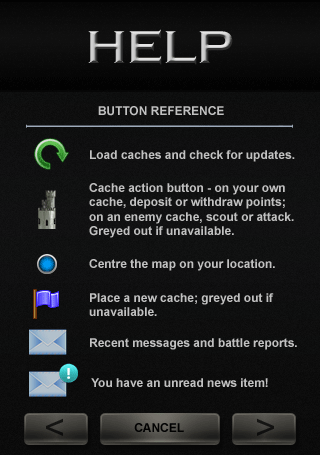
\includegraphics[width=0.25\textwidth]{images/help_mockup}
	\caption{Button reference in the help section.}
	\label{help_mockup}
	\end{center}
	\vspace{40pt}
\end{wrapfigure}

While designing the interface, it was important at all times to consider ease of use for users of various levels of familiarity with the system. Our domain analysis had highlighted the importance of intuitiveness in a system and of required functions being easily accessible (23 Cats, 2012:5-7); for this reason we have tried at all times to make the interface clear, and have also included a help screen should the user ever require it (see fig 2.1). Bell (1987) highlights the role of a well designed user interface in reducing errors, and to this end several of the features of our app were tested on potential users during development. In particular, it had originally been decided to disable the android back button within the app to give us greater control over which screens the user could access at any point in time. However, our users found the lack of a back button difficult to get used to, and so its functionality has been incorporated into the application wherever possible.

\begin{wrapfigure}{r}{0.25\textwidth}
	\vspace{-25pt}
	\begin{center}
	
\includegraphics[width=0.18\textwidth]{images/flags_greye}
	\caption{The available (left) and unavailable (right) place cache button.}
	\label{flags_greye}
	\end{center}
	\vspace{-10pt}
\end{wrapfigure}

To further the ease of use of the Fortitude Application, buttons which perform a specific action will be greyed out when the action is not available. These include, for example, the ``place cache'' button which would be greyed out if the user was too close to an existing cache, shown right in fig 2.2. The greyed out flag would perform no action if it was clicked on.

Every screen on the application has been designed to satisfy non-functional requirement 5.3.7: Interface Style Uniformity by using a consistent colour scheme and placement of buttons and headers. The colour scheme has been chosen to be silver or white on black, as the monochrome black and white is easy for all people to read, including those who are colour blind.

Non-functional requirement 5.3.9: Interface Feedback Delay requires that the app provide a fast response to user input; this has been achieved by the use of separate images for on-press actions, as shown below in fig 2.3. The change in luminosity of the buttons when pressed ensures the user is aware that the system has received their request.

\begin{figure}[ht]
	\vspace{-10pt}
	\begin{center}
	
\includegraphics[width=0.3\textwidth]{images/buttons}
	\vspace{-10pt}
	\caption{An inactive button (left) and an active button (right).}
	\label{buttons}
	\end{center}
\end{figure}

\subsubsection{Fortitude-game.co.uk Website}

The website is a supporting feature to the Fortitude application. With its larger dimensions and lack of battery and data restraints, the website can incorporate much of the functionality that is not feasible to include on the app, such as 5.3.6: Activity Recording. This serves to make the app simpler and therefore more user friendly without compromising the scope of the system.

The website is also the chosen interface for administrators to use to interact with the app as specified by a variety of requirements including 5.1.3: Administrator Accounts. The web interface provides an easy to access alternative to bespoke software and is not device dependant in the way that the app itself is; as administrators may not have an Android device, no administrator actions are incorporated into the app itself.

\begin{figure}[ht]
	\begin{center}
	
\includegraphics[width=0.9\textwidth]{images/website_header_background}
	\caption{The header image, an example of the more complex graphics used in the website. The white bordered box will hold the navigation.}
	\label{website_header_background}
	\end{center}
	\vspace{-20pt}
\end{figure}

\begin{wrapfigure}{r}{0.25\textwidth}
	\vspace{-15pt}
	\begin{center}
	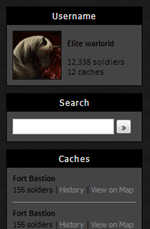
\includegraphics[width=0.25\textwidth]{images/sidebar_modules}
	\caption{Examples of the individual ‘modules’ that comprise the website (in this instance, the sidebar).}
	\label{sidebar_modules}
	\end{center}
	\vspace{-20pt}
\end{wrapfigure}

Requirement 5.4.8: Website Application Style Uniformity requires the overall design of the website to match that of the application. This has been achieved with the use of the same white on black colour scheme and recurring details such as Fortitude logo of two flags flying over a castle tower and the navigation menu of the website echoing the message box of the app. However, the simplicity of design used on the app has been expanded upon in the website with the addition of more dramatic imagery (see fig 2.4). This makes the website visually appealing without sacrificing ease of use as would be the case should such graphics be incorporated into the app.

Commonly accessed areas of the website, such as the sidebar and the home page, are organised into `modules', as in fig 2.5, making information quickly and easily identifiable. It also provides an excellent template for adaptation; though out of scope for this project, users could in future personalise their interaction with the website through selecting which of these modules to display on the side bar and home page. 


As in the application, the fortitude-game.co.uk website provides feedback in order to increase the efficiency with which the user can interact with the website and to reduce errors. This feedback can be in the form of data validation, such as in fig 2.6, or providing  a loading message while a section of the page loads. For more critical data entry, such as an administrator creating a new cache, the user is presented with a summary page of the information they have entered and must confirm it is correct before the new data is stored. This provides confirmation of the action as well as giving the user the chance to reduce errors, a key requirement of a well designed user interface.

\begin{wrapfigure}[6]{l}{0.3\textwidth}
	\vspace{-20pt}
	\begin{center}
	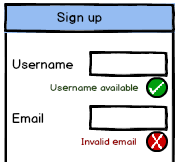
\includegraphics[width=0.25\textwidth]{images/sign_up_wireframe}
	\caption{Wireframe showing user feedback when creating an account.}
	\label{sign_up_wireframe}
	\end{center}
\end{wrapfigure}

The website also provides feedback if an error occurs – the most common is anticipated to be that the user has javascript disabled, which will cause every javascript dependent element of the site to be replaced with a placeholder informing the user that javascript is required and of the correct size and shape to avoid disturbing the rest of the website layout.
\vspace{80pt}
\subsection{Process Descriptions}

\subsubsection{Opening the application}
The process of the user opening the application is designed to be quick and efficient. To this end, the user will be taken straight to the main screen from the splash screen if they are already signed in to the application, to avoid the hassle of entering their login details again.

The choice between the main and unactivated main screens reflects functional requirement 5.1.2: Account activation, whereby users who have not activated their accounts are given limited functionality while using the application. The screen to create a new user leads directly to this unactivated main screen; once the user has activated their account through the verification email sent to them on creating the account, they will be taken to the main screen the next time they open the app. As per functional requirement 5.1.4: Resend activation email, the user is given the opportunity from the unactivated main screen to request a second email be sent should they have not received the first.

\begin{figure}[h!]
\centering
\begin{tabular}{cc}
	\begin{minipage}{0.4\textwidth}
		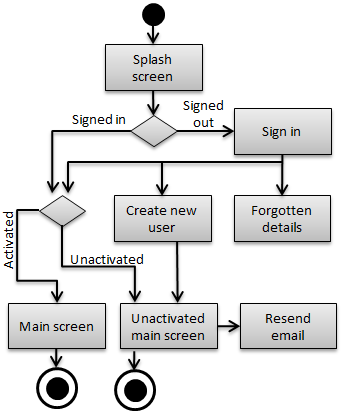
\includegraphics[width=1\textwidth]{images/opening_app}
		\caption{Screen map for the process of opening the app.}
		\label{opening_app}
	\end{minipage}
	\begin{minipage}{0.5\textwidth}
		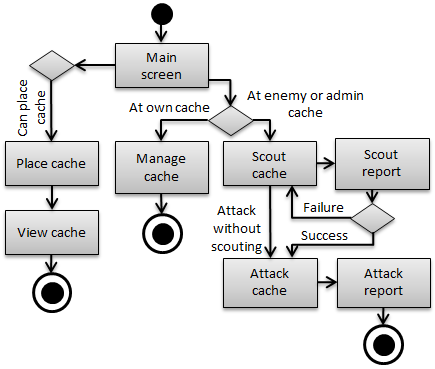
\includegraphics[width=1\textwidth]{images/key_actions}
	\caption{Screen map for key game actions.}
	\label{key_actions}
	\end{minipage}
\end{tabular}
\vspace{-20pt}
\end{figure}

\newpage
\subsubsection{Performing key game actions}

There are three main actions key to the game of Fortitude. They are creating caches (place cache), defending caches (manage cache) and conquering caches (scout then attack cache), and all are easily accessible through the main screen. Each action requires the user to be present at the cache/location of new cache, and the buttons calling these commands will be greyed out if this is not the case (see fig 2.2). The choice to combine both managing a cache the user owns – that is, depositing or withdrawing points in the cache to defend it against attack, or withdrawing all points to abandon the cache – and attacking or scouting an enemy cache into one ‘cache action’ button was taken to simplify the process of playing the game for the user, while at the same time reducing redundancy and clutter on the main screen.

\subsubsection{Viewing caches}

\begin{wrapfigure}{r}{0.5\textwidth}
	\vspace{-85pt}
	\begin{center}
	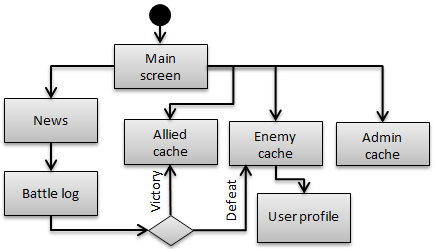
\includegraphics[width=0.5\textwidth]{images/viewing_caches}
	\caption{Screen map for key game actions.}
	\label{viewing_caches}
	\vspace{-10pt}
	\end{center}
\end{wrapfigure}
The ability to view caches is also integral to the above three actions, and is available at all times from the main screen (see fig 2.15) – the user does not have to be present at a cache to view its details. This is to enable the user to plan their game strategy, and keep track of their caches, and includes an option for the user to plan a route to the cache (functional requirement 5.3.4 Path finding) which will display on the map on the main screen (see fig 2.14). Beyond this, no game functions can be performed from viewing a cache – this must be done through the cache action button when physically present at the cache. However, the user profile of an enemy cache’s owner can be viewed, and caches can be reported to admins (see 2.2.5).

The user also has the option to view a cache from a battle report sent to their notifications after another player has attacked one of their caches. When taken to the cache in question; if their defenders were victorious they will see an allied cache, but if the attackers won they will see an enemy cache.

\subsubsection{Reading and sending messages}
\begin{wrapfigure}{rl}{0.4\textwidth}
	\vspace{-75pt}
	\begin{center}
	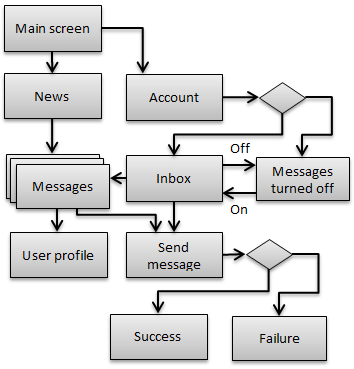
\includegraphics[width=0.4\textwidth]{images/sending_messages}
	\caption{Screen map for key game actions.}
	\label{sending_messages}
	\end{center}
\end{wrapfigure}
The primary way that users interact with other users other than directly attacking their caches is by sending messages. This allows users to form alliances and build complex battle strategies within the game and satisfies requirement 5.4.1: User communication. From the inbox, users are also given the option to turn the messaging system off if they do not wish to use it. When sending a message, the user will be informed through a messagebox if the recipient has messages turned off – or if an error prevented the message being sent. This is to ensure the user is kept informed about their actions and does not send multiple messages believing the previous ones to have failed. Users are also given the chance to report communications or block users if they wish to (see 2.2.5).

\subsubsection{Reporting and Blocking}
\begin{wrapfigure}{r}{0.25\textwidth}
	\vspace{-20pt}
	\begin{center}
	
\includegraphics[width=0.25\textwidth]{images/report_mockup}
	\caption{Screen map for key game actions.}
	\label{report_mockup}
	\end{center}
	\vspace{-130pt}
\end{wrapfigure}

Requirements 5.2.2: Cache reporting and 5.4.2: Communication reporting both require the user to be able to alert the administrators of certain caches, users or communications. This is anticipated to include a cache placed on a private or otherwise inaccessible location, or users behaving inappropriately towards others, and will be handled through a single report form (fig 2.8). The subject line of the report form is automatically filled in according to the screen from which the user decided to report (see fig 2.9), and a copy of the offending message, user profile or cache is sent along with the message to give administrators as much information as possible.

\begin{centering}
\begin{figure}[ht]
	\begin{minipage}{0.5\textwidth}
	\begin{tabularx}{\textwidth}{| X | X |}
		\hline
		Outlaw camp & Outlaw camp \\
		Enemy cache & User owned cache \\
		Allied cache & User owned cache \\
		Message & User communication \\
		User profile & User profile \\
		\hline
	\end{tabularx}
	\caption{Screens from which a user can report,
	and the corresponding subject line.}
	\label{report_table}
	\end{minipage}
\end{figure}
\end{centering}

Blocking users ensures that a user will receive no messages from the user they have blocked, though both users will be able to view and attack each other’s caches. Users can view a list of blocked users from their inbox, and from here can block or unblock a user. Blocking a user can  also be done from the user profile.

\subsubsection{Administrators acting on user request}

\begin{wrapfigure}{l}{0.5\textwidth}
	\vspace{-20pt}
	\begin{center}
	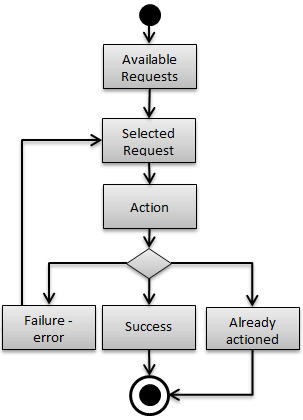
\includegraphics[width=0.35\textwidth]{images/admins_acting}
	\caption{Administrators acting on a user request.}
	\label{admins_acting}
	\end{center}
	\vspace{-40pt}
\end{wrapfigure}

User requests submitted from the application are always in the form of a report, as detailed above in 2.2.5. However, a user may submit other requests through the website, including a request to delete their account or a support question sent through the help page. All of these requests must be acted upon by an administrator; this is done through the admin section of the website. Certain requests, such as deleting the account, must be confirmed by the user before they are sent to the administrator; this is done by an email being sent to the user after they have initiated the request. The email contains a link to confirm the request; clicking on this link generates a request for the administrators act upon.

Here, administrators are able to see a page of all available requests, a request being available if it is not being worked on by another administrator at the time. The administrator selects a request (thereby removing it from the available requests page visible to all admins) and performs an action on it, which may be to complete the request or to flag the request if it cannot be completed at that point or by that administrator. The administrator will be informed of the result of their action and any details about a failure, such that the administrator can correct their mistake or flag the request. In the unlikely instance that two administrators try to act upon the same request (although occurrences of this are minimised by the request being removed from the available requests page), the first action will be performed and the second administrator informed of this when they submit their own action. Once acted upon, requests will be accessible through a ‘past requests’ page.

\subsubsection{Miscellaneous other}

\begin{wrapfigure}{r}{0.25\textwidth}
	\vspace{-40pt}
	\begin{center}
	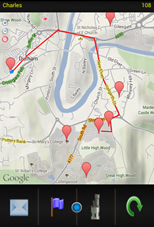
\includegraphics[width=0.25\textwidth]{images/route_mapping}
	\caption{Displaying a route to a cache.}
	\label{route_mapping}
	\end{center}
	\vspace{-80pt}
\end{wrapfigure}

Signing out is done from the user account settings, accessed from clicking on the status bar on the main screen.

Special placement caches are not available by user request; an icon relating to the cache will appear on the screen if the user has the application open while at the correct location. After clicking on this icon, the user will be asked to accept or reject the reward for finding the cache, without having to conquer the cache to receive it.

Routes to caches are shown on the main map as a thick red line (see fig 2.14). They can be planned from any type of ‘view cache’ screen and are cleared through the account menu. Routes are also cleared before each route is mapped, such that there can only be one route displaying on the map at any given time. The route is planned from the user's current location, which is updated when the user presses the refresh button.
\vspace{30pt}

\subsection{User Interface Design – Fortitude Application}

\subsubsection{Main screen}

\begin{figure}[ht]
	\begin{center}
	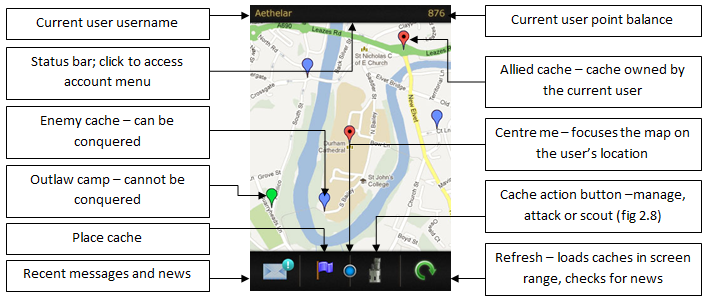
\includegraphics[width=0.9\textwidth]{images/main_screen}
	\caption{The main screen of the Fortitude application.}
	\label{main_screen}
	\end{center}
\end{figure}

The main screen is the core of the Fortitude application through which all key features are easily accessible. These are split into features relating to playing the game, grouped in the action bar at the bottom of the screen, and features relating to providing the user with information or allowing them to access their account, grouped in the status bar at the top of the screen. When clicked, this status bar leads the user to their account menu through which they can sign out, access their message inbox, or view the help screen. The status bar also displays the point balance available to the user; as points are required for core actions, it is important that this information is very visible, as specified by functional requirement 5.2.1: Account balance.

\begin{wrapfigure}{r}{0.25\textwidth}
	\vspace{-45pt}
	\begin{center}
	
\includegraphics[width=0.25\textwidth]{images/news_icons}
	\caption{The 'Recent news' icon and (right) with notification.}
	\label{news_icons}
	\end{center}
	\vspace{15pt}
\end{wrapfigure}

The action buttons relating to game play are grouped at the bottom of the screen, where it is most ergonomic for the user to access them. Each button is clearly distinct and, where appropriate, contains easily discernible extra information – such as the place cache and cache action buttons being greyed out when unavailable (see fig 2.2) and the recent news having a notification symbol to indicate unread news (fig 2.16). 

\begin{wrapfigure}{l}{0.2\textwidth}
	\vspace{-20pt}
	\begin{center}
	
\includegraphics[width=0.15\textwidth]{images/grey_pins}
	\caption{The pins are easy to tell apart without colour.}
	\label{grey_pins}
	\end{center}
	\vspace{-20pt}
\end{wrapfigure}

The main area of the home screen is the map, chosen as a very user friendly interface for the game and fulfilling several requirements including 5.3.1: Display location and 5.2.3: Nearby caches. Caches are clearly distinguished with different coloured pins to differentiate between admin, allied and enemy caches, as per requirement 5.2.3: Cache ownership and 5.2.26: Distinguishing cache owners; the colours are chosen to account for those with colour blindness (see fig 2.17). The map itself is controlled with the touch screen, using swipe or drag to navigate and pinch to zoom (zoom required by 5.3.3: Map zooming). To reduce data usage as per non-functional requirement 5.2.30: Data usage, adjusting the map view by zoom or location will not load the caches for that area of the map. This will be done by the green refresh arrow on the right of the status bar which also updates point balance, a route to a cache if active, and recent news feed as required.

\subsubsection{Unactivated main screen}

\begin{wrapfigure}{r}{0.25\textwidth}
	\vspace{-50pt}
	\begin{center}
	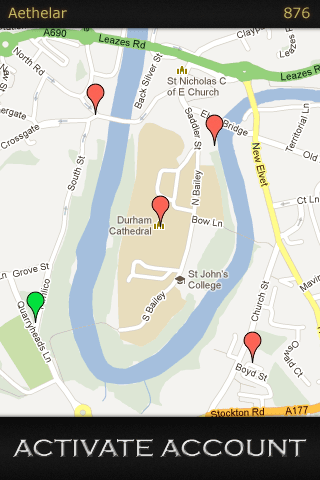
\includegraphics[width=0.25\textwidth]{images/unauthorised_main_mockup}
	\caption{Unactivated main screen.}
	\label{unactivated_main}
	\end{center}
	\vspace{-50pt}
\end{wrapfigure}

The main screen for the unactived user is identical in appearance to the main screen for an activated user (see fig 2.15), with the only difference being in the bottom bar. On the standard main screen this contains several buttons linking to features or actions which are not available to unactivated users – as specified by functional requirement 5.1.2: Account Activation. Here, this bar is replaced by a banner reminding users to activate their account; when clicked, this banner leads to the resend activation email page.

All other features have the same functionality as the main screen. The only difference is in navigating the map; on the unactivated account, each request to load a new view of the map also loads every cache within that view. This is because the unactivated user is not able to refresh the screen, as this button is located on the action bar which is not available here.

\subsubsection{User text input}

Many screens make use of text the user has input, most notably those involved with signing in or creating a new account (see fig 2.7) as well as sending messages to users (fig 2.19) or reports to administrators. Text input is handled through the on screen keyboard that is standard on an android phone (see fig 2.20). 
\vspace{0pt}
\begin{figure}[h!]
\centering
\begin{tabular}{cc}
	\begin{minipage}{0.3\textwidth}
		\begin{center}
		\begin{minipage}{0.83\textwidth}
		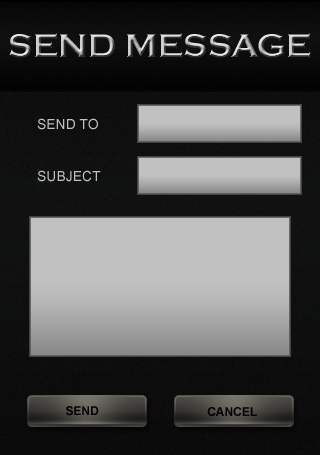
\includegraphics[width=\textwidth]{images/send_message_mockup}
		\caption{Send message screen, showing user text input fields.}
		\label{send_message}
		\end{minipage}
		\end{center}
	\end{minipage}
	\begin{minipage}{0.3\textwidth}
		\begin{center}
		\begin{minipage}{0.79\textwidth}
		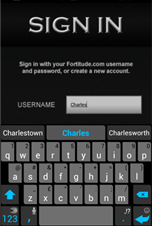
\includegraphics[width=\textwidth]{images/onscreen_keyboard}
		\caption{Using the on screen keyboard to sign in.}
		\label{onscreen_keyboard}
		\end{minipage}
		\end{center}
	\end{minipage}
	\begin{minipage}{0.3\textwidth}
		\begin{center}
		\begin{minipage}{0.83\textwidth}
		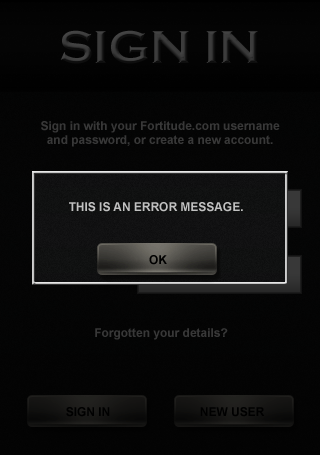
\includegraphics[width=\textwidth]{images/message_box_in_use_mockup}
		\caption{An example of a message box displaying an error message.}
		\label{message_box}
		\end{minipage}
		\end{center}
	\end{minipage}
\end{tabular}
\vspace{-0pt}
\end{figure}

Should the user input invalid information, such as incorrect login details, then an error message will be displayed (see fig 2.21). The screen behind this message will be dimmed to ensure the message is clearly visible. A similar design will be used for all message alerts to the user, such as error messages, status messages (for example ‘connecting to server’) or confirmation messages, which may have two options for the user to choose between (see fig 2.22)

\begin{wrapfigure}{r}{0.25\textwidth}
	\vspace{-30pt}
	\begin{center}
	
\includegraphics[width=0.25\textwidth]{images/message_box_question_mockup}
	\caption{A message box with two options.}
	\label{message_box_two_options}
	\end{center}
	\vspace{-30pt}
\end{wrapfigure}

Message boxes and text input fields are always of a consistent design to make them easy for the user to identify, though message boxes may stretch to contain longer messages.

\subsubsection{Menu and Information screens}

Many screens in the application give the user a set of options or provide some form of information. Viewing caches is one such example, as is the account menu (fig 2.23). The primary aim of these screens is to make the information as clear as possible to the users while at the same time making efficient use of space, so that the user does not have to click through multiple nested menus to access any feature. There is also consistency across screens; the ‘cancel’ button, for example, is always either the central bottom button or the bottom right.

The use of images when viewing a cache provides not only aesthetic appeal, but also serves a functional purpose. With different images used for enemy caches, allied caches and administrator caches, it is easy to identify from the cache screen what type of cache is being viewed; again, this refers back to requirement 5.2.26: Distinguishing caches.
\newpage
\vspace{-20pt}
\begin{figure}[h!]
\centering
\begin{tabular}{cc}
	\begin{minipage}{0.3\textwidth}
		\begin{center}
		\begin{minipage}{0.83\textwidth}
		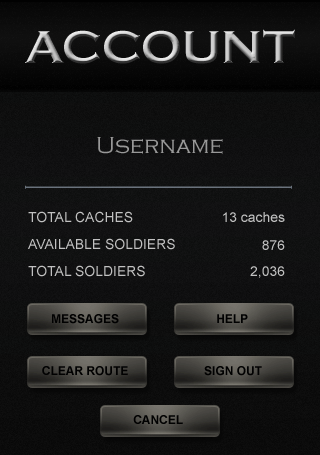
\includegraphics[width=\textwidth]{images/account_mockup}
	\caption{The user's account menu.}
	\label{account}
		\end{minipage}
		\end{center}
	\end{minipage}
	
	\begin{minipage}{0.3\textwidth}
		\begin{center}
		\begin{minipage}{0.83\textwidth}
		
\includegraphics[width=\textwidth]{images/enemy_cache_mockup}
	\caption{Viewing an enemy cache.}
		\end{minipage}
		\end{center}
	\end{minipage}
	\begin{minipage}{0.3\textwidth}
		\begin{center}
		\begin{minipage}{0.83\textwidth}
		
\includegraphics[width=\textwidth]{images/news_mockup}
	\caption{A page of items in the recent news.}
		\end{minipage}
		\end{center}
	\end{minipage}
\end{tabular}
\vspace{-0pt}
\end{figure}

\subsubsection{List screens}

Lists are used for displaying news items and messages in the inbox. Each screen displays several items on a single screen with forward and back buttons at the bottom of the screen to view the next page of items. This helps to limit data usage and loading times for the user whilst also providing an easy to navigate, well ordered system of displaying the items.

The use of icons to distinguish between types of items – battle reports and news icons, for example – makes it easier to take the list as a whole in without difficulty, and fading the icons of items which are not new helps the user find the important information with greater ease (as shown in the bottom 3 icons of fig 2.25).

\subsubsection{Action screens}

\begin{figure}[h!]
\centering
\begin{tabular}{cc}
	\begin{minipage}{0.3\textwidth}
		\begin{center}
		\begin{minipage}{0.83\textwidth}
		
\includegraphics[width=\textwidth]{images/attack_cache_mockup}
	\caption{Attacking a cache.}
		\label{attack_cache}
		\end{minipage}
		\end{center}
	\end{minipage}
	\begin{minipage}{0.3\textwidth}
		\begin{center}
		\begin{minipage}{0.83\textwidth}
		
\includegraphics[width=\textwidth]{images/scout_cache_mockup}
	\caption{Scouting a cache.}
		\label{scouting_cache}
		\end{minipage}
		\end{center}
	\end{minipage}
	\begin{minipage}{0.3\textwidth}
		\begin{center}
		\begin{minipage}{0.83\textwidth}
		
\includegraphics[width=\textwidth]{images/place_cache_mockup}
	\caption{Placing a cache.}
		\label{placing_cache}
		\end{minipage}
		\end{center}
	\end{minipage}
\end{tabular}
\vspace{-0pt}
\end{figure}

 Screens involving direct interaction with caches, such as attacking, managing (withdrawing or depositing soldiers) or placing caches are of a similar layout to provide consistency throughout the game. The screens are clearly differentiated by the use of different images – such as a charging soldier on the attack screen versus a sneaking soldier on the scouting screen (see figs 2.26 and 2.27) as well as by the action title being clearly displayed. The name of the cache involved is also clearly displayed on the screen. Any time that user input is required in these screens it is done in such a way as to restrict the values of possible user input to those which are known to be valid, such as using a slider to change the number of soldiers committed to an action or choosing between a choice of names when creating a cache (see fig 2.28). This is to make the process of game play as quick and error free as possible.

\subsubsection{Reporting results}

Any action with an unknown outcome is reported to the user using a screen of the same design, again to make the app consistent and increase the user’s familiarity with how it works and where information is displayed. Where relevant, the image of the report screen reflects the outcome – such as a scroll for a successful scouting mission versus a tomb stone for a failed one (fig 2.29). As ever, this is both for aesthetic reasons and to communicate the necessary information to the user clearly and quickly.

A similar report screen is also accessible from the news feed for the report of a cache the user owns which has been attacked by another player. This screen differs in that the name of the cache is more prominent and there is a link to view the cache on the map; this is required to identify the cache as the user may not be present at the cache’s location.

\begin{figure}[h!]
\centering
\begin{tabular}{cc}
	\begin{minipage}{0.3\textwidth}
		\begin{center}
		\begin{minipage}{0.83\textwidth}
		
\includegraphics[width=\textwidth]{images/total_wipeout}
	\caption{Unsuccessful scout mission report.}
		\label{attack_cache}
		\end{minipage}
		\end{center}
	\end{minipage}
	\begin{minipage}{0.3\textwidth}
		\begin{center}
		\begin{minipage}{0.83\textwidth}
		
\includegraphics[width=\textwidth]{images/battle_report_mockup}
	\caption{Reporting a battle result.}
		\label{scouting_cache}
		\end{minipage}
		\end{center}
	\end{minipage}
	\begin{minipage}{0.3\textwidth}
		\begin{center}
		\begin{minipage}{0.83\textwidth}
		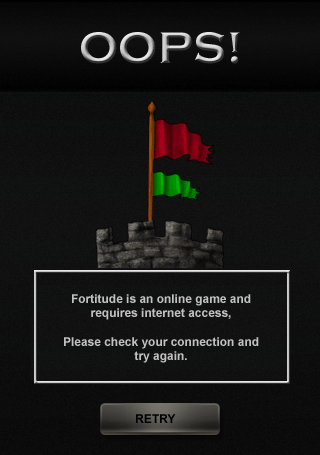
\includegraphics[width=\textwidth]{images/error_mockup}
	\caption{An error caused by lack of internet connection.}
		\end{minipage}
		\end{center}
	\end{minipage}
	
\end{tabular}
\vspace{-0pt}
\end{figure}

\subsubsection{Static screen}

The final type of screen is a static screen. This is one not designed for much user interaction; the full screen is comprised of a single image or static text, such as the Fortitude logo on the splash screen or the help screens (fig 2.1). The splash screen itself has no buttons for the user to progress, as the app will automatically move on once it has loaded. Other static screens, such as the help screens, have a button to move on from this screen.

Static screens are used for errors which cause the app itself to be unplayable – the most common of which would be the user not having internet connection available (see fig 2.31) – and the user will be unable to move from this screen until the error has resolved. A static screen is also used for when a user comes across a special placement cache, with which they cannot interact but must either accept or reject the prize.

With the exception of the help screens, static screens cannot be called by the user; they are initiated by the server and used to send a message to the user that cannot be ignored or minimised until normal game play can resume.

\subsection{User Interface Design – Fortitude-game.co.uk}

\subsubsection{Site Layout}

The visual design of the website was chosen to reflect the dramatic battle-driven nature of the game of Fortitude. It clearly echoes the app in its sombre colour scheme of black, white and greys, and the use of the two flags image used as Fortitude’s logo (see fig 2.4). The choice of a more serious design both in the website and the app is to reflect the strategic and ‘epic’ style of game that Fortitude is, appealing to players of all ages.

\begin{wrapfigure}{l}{0.6\textwidth}
	\vspace{-30pt}
	\begin{center}
	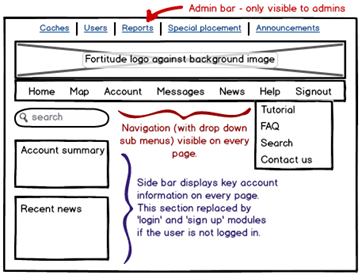
\includegraphics[width=0.6\textwidth]{images/website_wireframe}
	\caption{Wireframe of the site layout with space left for page content. The image used in the header is shown previously in figure ~\ref{fig:website_header} on page~\pageref{fig:website_header}.}
	\label{website_wireframe}
	\end{center}
	\vspace{-20pt}
\end{wrapfigure}

The basic structure of the website is for the page to be divided into three, with the top area containing navigation (including administrator links), the sidebar to the left containing key information and the larger area to the right displaying the page content for each page (see fig 2.32). Both the sidebar to the left and the main page content of the home page use modules to display content, making the information easily and quickly accessible. The administration links have been placed above the main page to ensure that they cannot interfere with the usual page content but are not sidelined and hard to get to; it is anticipated that administrators would mainly use the website for admin purposes, and so need the links to be clearly visible. These links will not be displayed for any user who is not an administrator; should they reach an administrator page, they will be shown a 404 page. Similarly, some pages are restricted to users; should a visitor who is not logged in attempt to view a page such as the account page, they will be redirected to the login/sign up screen.

The use of drop down sub menus is important to increase ease of navigation, enabling users to quickly reach areas of the website without over cluttering the top bar itself. However, as not all devices have a hover feature (such as tablets or phones), no area of the website will only be accessible through these sub menus.

\subsubsection{Site Content}

The content of the website will in many cases mimic that of the app, though in greater depth or with greater functionality – for example, the user can view caches on a map as they can through the phone, but can also apply a filter to display only their own or only enemy caches, as per requirement 5.4.7: Overview Map (see fig 2.33). In addition, some functionality is only available through the website – such as the ability to search for a user or cache by name, or the ability to view an activity log of recent activity associated with that account, specified in requirement 5.3.6: Activity Recording. Certain content, such as the home screen and site news, is visible to all whether logged in or not so as to give potential users a feel for the game and encourage them to sign up and participate. Other areas will redirect the user to the Login page which consists of two modules, one to log in and one to sign up. These modules will also be visible on the side bar at all times unless the user is logged in, in which case the side bar will display key information.

\subsubsection{The Map}

\begin{wrapfigure}{r}{0.6\textwidth}
\vspace{-40pt}
	\begin{center}
	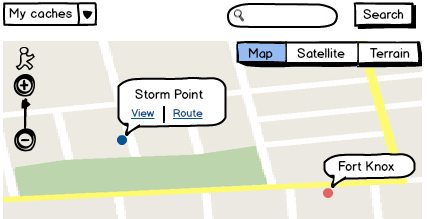
\includegraphics[width=0.6\textwidth]{images/map_wireframe}
	\caption{Wireframe of the map and controls}
	\label{map_wireframe}
	\end{center}
	\vspace{-10pt}
\end{wrapfigure}

The map will use the familiar google maps interface with zoom, street view, and different types of map (satellite, terrain etc). The user can search the map by location, username (ie all caches owned by a certain user) or cache name; should multiple caches with the same name be found, both would be displayed on the map (and the zoom adjusted until both were visible), and the user could zoom in on the correct one. The option to filter caches is done through a drop down menu with filters including ‘All caches’, ‘My caches’, ‘Enemy caches’, and ‘Outlaw camps’ (non-player caches). Updating the map by either filtering or searching is done asynchronously, providing a much smoother experience for the user without having to reload the page each time a request is sent. Different types of caches are distinguished as on the app by colour and the presence of a dot, such that colour blind people can also tell caches apart. A cache displays its name and, when clicked on, choices to view the cache details or plan a route to it; this option will bring up a dialogue box asking for the location to plan the route from.

\subsubsection{Sidebar}

As mentioned previously in the Design Methodology (2.1.2), users will in future be able to personalise sections of the website including the sidebar to display the modules most appropriate to them. Until such a point, the sidebar will display to a logged in user a search bar, an account summary, a list of the user’s five most active caches – determined by the cache with the greatest frequency of events in its history – and a list of the user’s five most recent events. If a user who is not logged in views the site, the sidebar will contain the search module as well as modules to log in or sign up.

\begin{wrapfigure}{l}{0.45\textwidth}
	\begin{center}
	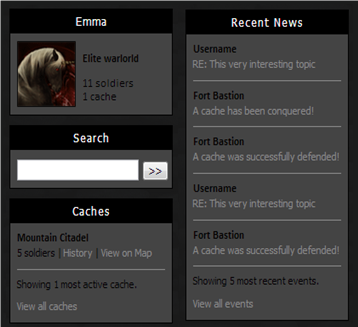
\includegraphics[width=0.45\textwidth]{images/sidebar}
	\caption{The key information displayed in the sidebar (recent news would be placed below rather than beside the other modules).}
	\label{sidebar}
	\end{center}
	\vspace{-100pt}
\end{wrapfigure}

The title ‘Elite Warlord’ in fig 2.34 Corresponds to the user’s level, determined by the number of caches they own. The avatar and user title serve little purpose as far as game play is concerned, but contribute towards personalising a user’s account and, in the levels, giving a tangible goal to aim for in the game.

\subsubsection{Administrator pages}

The administrator features of the website are accessible through the navigation links at the top of the screen, which are only visible to users logged in as administrators. These are highlighted in green, the colour making them stand out and separate from the rest of the website. The tasks that can be completed from each page are shown below in fig 2.36. 
\vspace{55pt}
\begin{figure}[ht]
	\begin{center}
	
\includegraphics[width=0.6\textwidth]{images/admin_bar}
	\caption{The administrator links. The bar itself extends horizontally to fill the page.}
	\label{admin_bar}
	\end{center}
\end{figure}
\begin{figure}[ht]
\begin{center}
\begin{tabular}{| p{0.22\textwidth} | p{0.68\textwidth} |}
	\hline
	Caches &
	View all caches, grouped under ‘user cache’ and ‘outlaw cache’. Includes options to view the history of or delete caches of any kind or add outlaw caches, as well as managing or editing outlaw caches. \\
	\hline
	Users &
	View the entire user list. Includes options to send users an official warning or other communication and to remove a user account (this would only be done by user request). \\
	\hline
	Reports &
	View all user requests that need to be acted on, and select individual requests to action. \\
	\hline
	Special Placement &
	Create and manage special placement caches. \\
	\hline
	Announcements &
	Post an announcement to the site (appears on the home page and news), and edit or delete old announcements. \\
	\hline
\end{tabular}
\caption {Tasks carried out by admins from each administrator page.}
\label{admin_page_tasks}
\end{center}
\end{figure}


Administrator pages can be roughly grouped into two types; those that involve viewing a database, and those that involve creating data such as a cache, special placement or announcement. Database style pages are laid out as shown in fig 2.37 (the header and sidebar sections are not shown, but are the same as the rest of the site). Filtering the database and commands such as creating new caches or, on the user request page, viewing past requests are linked from the top of the page for easy access, and the database is grouped by a tab system into the types of database. This avoids having redundant fields in an entry – such as the ‘owner’ field for an outlaw camp entry. The administrator cannot ever see the whole database on one page; they are originally shown only the filter section and must access the database by running a query from here. Should the query be too large, the administrator will be requested to narrow down the filter.

\begin{figure}[h!]
	\begin{center}
	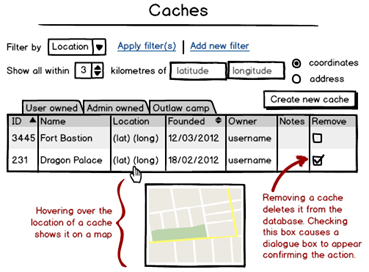
\includegraphics[width=0.6\textwidth]{images/caches_wireframe}
	\caption{Wireframe example of a database page, here managing caches with a location filter selected.}
	\label{caches_wireframe}
	\end{center}
\end{figure}

Creating data is handled through a form interface which, despite its simple design, is arguably the best method of data input for users (Dix, Finlay et al, 1993: PAGE NUMBER). The form provides user feedback for incorrect or invalid data entries in the same way as creating a user account would (see section 2.1.2).

%\subsection{User Interfaces}
%\lipsum[141-160]
%\subsection{Process Descriptions}
%\lipsum[61-80]
%\newpage
%\newcolumntype{C}[1]{>{\Centering}p{#1}}
\def\TabS#1#2{\small\tabular{#1}\rule[-1.5mm]{0pt}{5mm}{#2}
    \rule[-2mm]{0pt}{2mm}\endtabular\hspace{-1mm}}
\def\TabM#1#2{\tabular{#1}\rule[-1.5mm]{0pt}{7mm}{#2}
    \rule[-3mm]{0pt}{4mm}\endtabular\hspace{-1mm}}
\def\TabA#1#2#3{\small\tabular{#1}\rule[-1.5mm]{0pt}{5mm}\textbf{#2}\\
    \hline\rule[0mm]{0pt}{4mm}#3
    \rule[-2mm]{0pt}{2mm}\endtabular}
\def\TabB#1#2#3{\small\tabular{c}\rule[-1.5mm]{0pt}{5mm}
    \textbf{{\tiny$\ll$}#1{\tiny$\gg$}}\\
    \hline\rule[0mm]{0pt}{4mm}\tabular{ll}#2\endtabular \\
    \hline\rule[0mm]{0pt}{4mm}\tabular{ll}#3\endtabular
    \rule[-2mm]{0pt}{2mm}\endtabular}
\seticonparams{entity}{
    shadow=false,
    fillcolor=blue!10,
    fillstyle=solid,
    framesep=0pt}

\setcounter{section}{2}
\section{Element Descriptions}
\setcounter{subsection}{-1}
\subsection{Architecture Overview}
\subsubsection{Top Level Design}
It was apparent from the briefing and requirements that the most suitable architecture for the system would be a client-server model. There will be a central server that stores persistent system related data, and performs the majority of the application logic. This server services requests from many client applications that handle user interaction and present information through a graphical user interface. A requirement of the application was also to provide a website as a second source of user interaction, which will be implemented using the central server.

The server and client may be conceptually divided into several modules. For the server, there is the \emph{Database Module} that manages reading from and modifying the persistent application data, the \emph{Logic Module} that handles game and system calculations, and the \emph{Web Interface} group which contains the \emph{API Module} for interacting with client applications, and the \emph{Website Module} for servicing the website HTTP requests. The client will be constructed to include a \emph{Request Module} for contacting the server and interpreting any responses, a \emph{Logic Module} that is aware of relevant aspects of the game state and performs client-relevant calculations, a \emph{Geolocation Module} for interaction with the Google APIs and the GPS sensor, and a \emph{Window Module} for the graphical user interface.

\begin{figure}[h!]
    \centering
    \begin{tabular}{c}
    \entity{server}[\TabA{c}{Centralized Server}{~\\[-3mm]
        \tabular{c}~\\[-10mm]
            \entity{database}[\TabS{c}{Database Module}]\\[8mm]
            \entity{serverlogic}[\TabS{c}{Logic Module}]\\[-3mm]
        \endtabular
        \hspace{5mm}
        \entity{web}[\TabA{c}{Web Interface}{~\\[-3mm]
            \entity{api}[\TabS{c}{API Module}]\\[2mm]
            \entity{website}[\TabS{c}{Website Module}]\\[-3mm] 
        }]\\[-3mm]
    }]
    \hspace{5mm}
    \entity{app}[\TabA{c}{Client Android Application}{~\\[3mm]
        \hspace{-5mm}
        \tabular{cc}
        \tabular{c}~\\[-10mm]
            \entity{request}[\TabS{c}{Request Module}]\\[8mm]
            \entity{applogic}[\TabS{c}{Logic Module}]\\[-3mm]
        \endtabular
        \hspace{2mm}
        \tabular{c}~\\[-10mm]
            \entity{window}[\TabS{c}{Window Module}]\\[8mm]
            \entity{geo}[\TabS{c}{Geolocation Module}]\\[-3mm]
        \endtabular\hspace{-3mm}
        \endtabular
        \\[3mm]
    }]
    \end{tabular}
    {\small
        \ncline[arrowscale=1.5]{<->}{database}{serverlogic}
        \nccurve[arrowscale=1.5,angleA=5,angleB=175]{<->}{serverlogic}{api}
        \nccurve[arrowscale=1.5,angleA=-5,angleB=-175]{<->}{serverlogic}{website}
        %\ncline[arrowscale=1.5]{->}{database}{web}
        \nccurve[arrowscale=1.5,angleA=0,angleB=180]{<->}{api}{request}
        \ncline[arrowscale=1.5]{<->}{request}{applogic}
        \nccurve[arrowscale=1.5,angleA=45,angleB=-135]{<->}{applogic}{window}
        %\ncline[arrowscale=1.5]{->}{request}{window}
        \ncline[arrowscale=1.5]{->}{geo}{applogic}
    }
    \caption{Data flow of the top level of the system, showing the application and server as clearly separated entities with internal modules that encapsulate distinct functionalities of the system.}
\end{figure}

As \emph{Figure 1} shows, the server and client have a similar overall structure. Both have a main contained logic processing module, a modifiable data source (the \emph{Database Module} for the server and the \emph{Request Module} for the client), and an interface (the \emph{API Module} and \emph{Website Module} for the server, and \emph{Window Module} for the client). This compartmentalisation of processes is intended to make both the server and client subsystems more expandable and maintainable while features are being implemented and testing performed. The interaction between modules is restricted to a small and manageable set of interfaces to help reduce the internal complexity of the system.

\subsection{Intermodule Dependencies}
\subsubsection{Database Module}
This module will be used extensively by the other modules in the server, so considerable effort has been invested in designing a clean and powerful interface. The module will abstract away interaction with the DBMS (Database Management System), making it possible to easily replace the DBMS used to support different platforms. For the Windows operating system the server will be running on top of the .NET CLR (Common Language Runtime), and will therefore have access to Microsoft's SQL Compact Edition Server. On Unix systems, the server will be using the Mono CLR implementation, and will therefore have to use an alternative DBMS such as SQLite. As well as supporting different DBMS connections and SQL dialects depending on the host system, the Database Module will also provide a simple interface to common SQL operations through the use of code generation. This will reduce the amount of errors produced through the use of poorly constructed SQL statements by delegating the validation task to the debugging facilities provided by the IDE (Integrated Development Environment) used while developing the server.

\begin{figure}[h!]
    \centering
    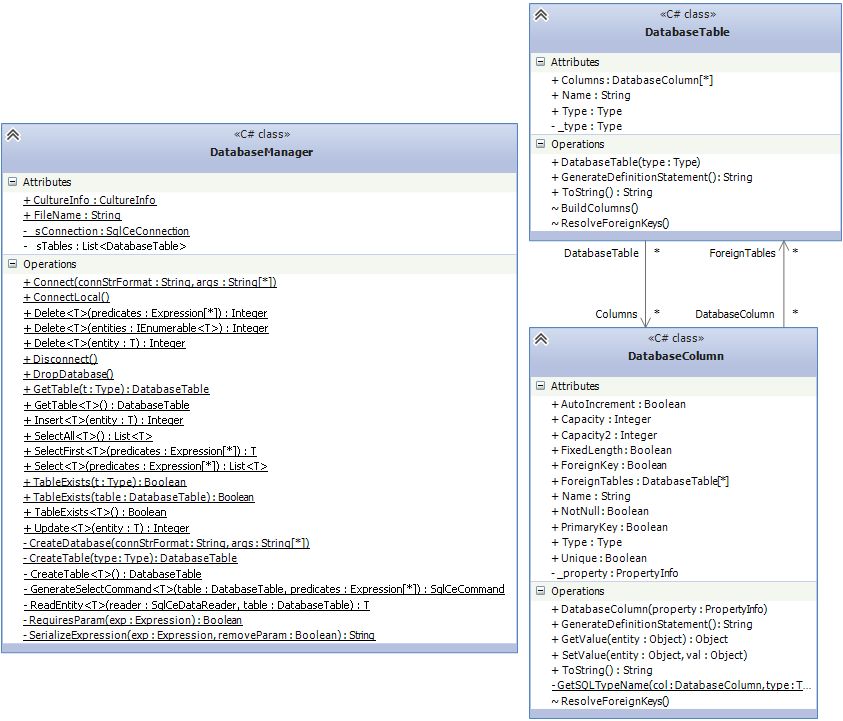
\includegraphics[width=\textwidth]{dbmancd}
    \caption{Class diagram for the main Database Module classes.}
\end{figure}

The three most important classes in the design are \emph{DatabaseTable}, \emph{DatabaseColumn} and \emph{DatabaseManager}. \emph{DatabaseTable} and \emph{DatabaseColumn} relate to the tables and columns respectively in the SqlCe (or Sqlite) database. This abstraction of the database structure is used internally in the database module for the generation of SQL statements and also when reading information supplied by the database management system. Database table is simply a named collection of columns, which can be automatically be constructed from a C$\sharp$ class which has a \emph{DatabaseEntity} attribute. When the server program initializes, all classes in the assembly are checked for this attribute. For each class that has one, a \emph{DatabaseTable} is constructed and stored for later use in the \emph{DatabaseManager}. If this table is not present in the actual database, a DDL statement is automatically generated to define and construct it. This application of assembly reflection and code generation greatly reduces the amount of work needed to implement and use new database entity types. All that is required is the definition of a C$\sharp$ class with the \emph{DatabaseEntity} attribute, and the fields to be stored marked with their respective attributes like the \emph{PrimaryKeyAttribute} and \emph{NotNullAttribute}. The class can then be immediately used in the code without manually adding it to any lists or writing a single line of SQL, and it will be stored in the database through a single call of \emph{DatabaseManager.Insert()}.

The \emph{DatabaseManager} class provides the bridge between the external DBMS and the internal representation of the database. It provides simple but useful functions to add, retrieve, and update items from the database. The aim with the design was to have a powerful interface without the need to write a single line of SQL when making a request. Hard coding SQL into the program would lead to a great deal more work when trying to support the two dialects used by the different management systems for each platform, and would require manual debugging instead of through the IDE's syntax validation. The query system will be implemented through the use of a translator that compiles C$\sharp$ LINQ (Language Integrated Query) expressions to SQL. Although an implementation of this functionality exists in the Microsoft implementation of .NET, the Mono one has no such feature. Therefore, the mechanism will have to be replicated specifically for this application.

\begin{figure}[h!]
    \centering
    \begin{tabular}{c}
        \entity{external}[\TabM{C{3cm}}{Other Server Modules}]
        \hspace{2cm}
        \entity{dbmodule}[\TabA{c}{Database Module}{
            \tabular{c}~\\[-2mm]
                \entity{translator}[\TabS{c}{Translator}]\\[3mm]
                \entity{reader}[\TabS{c}{Object Reader}]\\[3mm]
            \endtabular
        }]
        \hspace{2cm}
        \entity{dbms}[\TabM{C{25mm}}{Database Management System}]
        \hspace{5mm}
        \tabular{c}
            ~\\[-1cm]
            \pnode(0.22,-0.4){db}
            \database[database]{2cm}{1cm}[fillstyle=solid,fillcolor=blue!10]
                {Database}[database]
        \endtabular
    \end{tabular}
    \nccurve[arrowscale=1.5,angleA=15,angleB=180]{->}{external}{translator}
    \naput[nrot=:U,npos=0.35]{LINQ}
    \nccurve[arrowscale=1.5,angleA=-15,angleB=180]{<-}{external}{reader}
    \nbput[nrot=:U,npos=0.42]{C$\sharp$ Objects}
    \nccurve[arrowscale=1.5,angleA=0,angleB=165]{->}{translator}{dbms}
    \naput[nrot=:U,npos=0.65]{SQL}
    \nccurve[arrowscale=1.5,angleA=0,angleB=-165]{<-}{reader}{dbms}
    \nbput[nrot=:U,npos=0.58]{Raw Data}
    \nccurve[arrowscale=1.5,angleA=0,angleB=180]{<->}{dbms}{db}
    \nbput[nrot=:U,npos=0.54]{\tiny Magic?}
    \caption{Diagram showing the data flow of the Database Module during a \emph{SELECT} statement.}
\end{figure}

\subsubsection{Logic Module}
The Logic Module will contain all critical algorithms related to game and overall system state. This will include the operations of account authentication, client location validation, cache attacking, and unit transactions. The module contains a set of core classes that abstract components of the game such as caches and players. Keeping the more intensive calculations in the system separated from the database and interface means they are easier to locate and profile, and unit tests can be produced more simply without having to unnecessarily incorporate unrelated components.

This module is centred around processing the main elements of the game; players, caches, and their interactions. The \emph{Account} and \emph{Player} classes, which are \emph{DatabaseEntity} types, represent the account details and game states respectively of a user. The separation of user data between the two classes is designed to match the conceptual difference, and also because users who have not been verified by email do not need \emph{Player} objects since they are unable to participate in the game. The \emph{Account} class will provide a wide array of static helper methods; to register a new user, validate an existing one, or promote a user to administrator status for example. The \emph{Cache} class is also a \emph{DatabaseEntity}, and represents a single cache. It provides a helper method \emph{FindNearby} that is used both to detect whether a player is close enough to scout or attack a cache, and also whether a cache is too close to where a user wishes to place a new one. The other notable method is \emph{Cache.Attack} where the battle calculation is performed, deciding whether a cache is defeated by the attacking army or if the defenders keep possession of the stronghold.

Authentication sessions and notifications are also managed in this module. The decision has been made to not store authentication sessions in the database, but rather in memory. Authentication sessions are quite volatile, in that they will be created and removed too frequently to warrant their storage in a sluggish but persistent structure like a database. They will be instead held in a dictionary structure, using the related account ID as a key for easy retrieval. Notifications are messages to users about a change in game state that may be of interest to them, or for messages sent to them by other users. These objects \emph{are} stored in the database, and so the \emph{Notification} class has the \emph{DatabaseEntity} attribute.

\begin{figure}[h!]
    \centering
    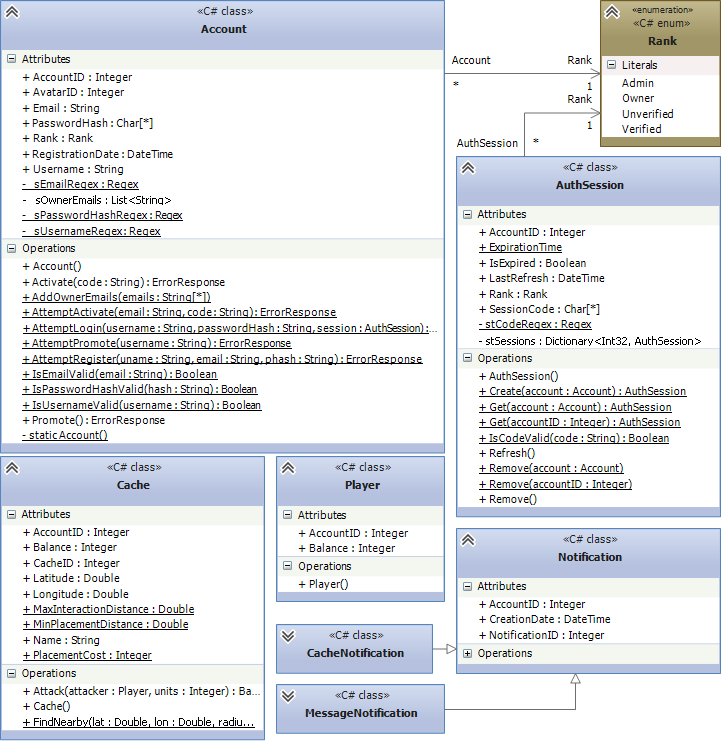
\includegraphics[width=\textwidth]{svlogiccd}
    \caption{Class diagram for the main Logic Module classes.}
\end{figure}

\subsubsection{Web Interface}
This module group is the interface in which incoming HTTP requests are processed and responded to. The requests come in two main categories; website resource requests and API requests. The website resource requests are from users browsing the website and requesting pages or static content such as images. These requests are directed towards the \emph{Website Module}, which processes them and responds with the requested content. API requests are sent by the client application, and will be routed to the \emph{API Module}. These requests are in the form of a command with a series of named parameters, and the response will be sent as a JSON (JavaScript Object Notation) object.

\begin{figure}[h!]
    \centering
    \begin{tabular}{c}
        \tabular{c}~\\[1cm]
            \entity{client}[\TabM{C{35mm}}{Client Application}]\\[15mm]
            \entity{browser}[\TabM{C{35mm}}{Client Web Browser}]
        \endtabular
        \hspace{2cm}
        \entity{web}[\TabA{c}{Web Interface}{
            \hspace{-3mm}
            \tabular{lr}~\\[-2mm]
                \entity{json}[\TabS{c}{JSON Serializer}]&\\[3mm]
                \entity{api}[\TabS{c}{API Manager}]&
                \entity{request}[\TabS{c}{Request Class}]\\[3mm]
                \entity{content}[\TabS{c}{Content Manager}]&
                \entity{script}[\TabS{c}{Scripted Page}]\\[3mm]
            \endtabular
            \hspace{-3mm}
        }]
        \hspace{1cm}
        \entity{logic}[\TabM{C{2cm}}{Logic Module}]\\[2cm]
    \end{tabular}
    {\small
        \nccurve[arrowscale=1.5,angleA=-5,angleB=180]{->}{client}{api}
        \nbput[nrot=:U,npos=0.45]{HTTP/GET}
        \nccurve[arrowscale=1.5,angleA=0,angleB=180]{->}{browser}{content}
        \naput[nrot=:U,npos=0.45]{HTTP/GET}
        \nccurve[arrowscale=1.5,angleA=0,angleB=180]{->}{api}{request}
        \nccurve[arrowscale=1.5,angleA=0,angleB=180]{->}{content}{script}
        \nccurve[arrowscale=1.5,angleA=90,angleB=0]{->}{request}{json}
        \nbput[nrot=:D,npos=0.5,labelsep=0mm]{\scriptsize Response Object}
        \nccurve[arrowscale=1.5,angleA=180,angleB=5]{->}{json}{client}
        \nbput[nrot=:D,npos=0.55]{JSON}
        \nccurve[arrowscale=1.5,angleA=0,angleB=180]{<->}{request}{logic}
        \nccurve[arrowscale=1.5,angleA=0,angleB=-90]{<->}{script}{logic}
        \nccurve[arrowscale=1.5,angleA=-115,angleB=-5]{->}{script}{browser}
        \nbput[nrot=:D,npos=0.4]{HTML}
    }
    \caption{Diagram showing the data flow of the \emph{Web Interface} module group.}
\end{figure}

\subsubsection{Website Module}
This submodule of the \emph{Web Interface} handles the delivery of web content such as HTML pages, style sheets, and images. The content is served from a resource directory local to the server program, which is updated during the program's runtime. It also allows dynamic web page generation through the use of inline C$\sharp$ scripts in the source HTML files. These scripts are used as a preprocessing language while constructing the page, so the resulting file sent to a user's web browser has content reflecting the current state of the game and the actions of the user. The inline preprocessor scripting system will be implemented specifically for this project, using code generation and .NET's ``compiler as a service'' facility. The choice to do this instead of simply using PHP or any other pre-existing CGI is so the scripts would have direct access to the server program and its components (this would be true because the scripts are actually contained within the server program itself). This would provide increased performance and would eliminate the need to produce an interface between the CGI and the server.

\subsubsection{API Module}
The second submodule of the \emph{Web Interface} group handles the interpretation and responses to requests from the client application. These requests arrive in the form of a specific command, and the named parameters required by that command. The module contains a class for each command, all extending a general \emph{Request} superclass that provides some facilities common to most requests such as authenticating the requesting user. After the request is processed, an object extending the \emph{Response} superclass is returned by the processing request class. This object is then serialized procedurally into a JSON object, which is sent as a reply to the requesting client. The separation of request and response types into classes has the standard benefits of reduced code dependencies and therefore complexity, and also allows requests (or responses) with similar functionalities to extend general abstract classes that implement them. JSON is used as a response format due to its small bandwidth footprint and how trivial it is to parse. It also opens up the possibility of using it with AJAX for the website implementation.

Assembly reflection will be used to automatically detect the corresponding class for each request, and then create an instance of it. All \emph{Request} classes will override a \emph{Respond} method with a \emph{Response} return type, which will be invoked upon instance creation.

\def\Req#1#2{\entity{a#1}[\TabS{C{45mm}}{#2Request}]\\[2mm]}
\def\Res#1#2{\entity{b#1}[\TabS{C{45mm}}{#2Response}]\\[6mm]}
\def\Con#1#2{\nccurve[arrowscale=2,angleA=0,angleB=180]{->}{a#1}{b#2}}

\begin{figure}[h!]
    \centering
    \tabular{c}
    \Req{ech}{Echo}
    \Req{act}{Activation}
    \Req{pas}{PasswordReset}
    \Req{reg}{Register}
    \Req{sen}{SendActivation}
    \Req{sta}{StartSession}
    \Req{uir}{UserInfo}
    \Req{usr}{UserStats}
    \Req{ucr}{UserCaches}
    \entity{loc}[\TabA{c}{Locational}{
        \hspace{-4mm}
        \tabular{c}~\\[-3mm]
        \Req{cac}{CacheTransaction}
        \Req{nea}{NearbyCaches}
        \Req{pla}{PlaceCache}
        \Req{att}{AttackCache}
        \Req{sco}{ScoutCache}
        \endtabular
        \hspace{-4mm}
    }]
    \endtabular \hspace{45mm}
    \tabular{c}
    \Res{ech}{Echo}
    \Res{res}{}
    \Res{ses}{SessionInfo}
    \Res{usi}{UserInfo}
    \Res{uss}{UserStats}
    \Res{cac}{CacheInfo}
    \Res{bat}{BattleReport}
    \Res{sco}{ScoutCache}
    \endtabular
    \Con{act}{res}
    \Con{att}{bat}
    \Con{cac}{res}
    \Con{ech}{ech}
    \Con{nea}{cac}
    \Con{pas}{res}
    \Con{pla}{cac}
    \Con{reg}{res}
    \Con{sco}{sco}
    \Con{sen}{res}
    \Con{sta}{ses}
    \Con{ucr}{cac}
    \Con{uir}{usi}
    \Con{usr}{uss}

    \caption{A list of each \emph{Request} and \emph{Response} type, and the relationships between them.}
\end{figure}

The \emph{Response} superclass has one mandatory attribute - a boolean marking whether the original request was successful or not. For all but one of the extending subclasses, this flag is set to true by default. The one class that doesn't is the \emph{ErrorResponse} class. This class also includes a \emph{String} attribute containing a message describing why the request failed. The mandatory inclusion of the \emph{success} boolean means the receiver of the response can tell if the response object will contain the desired output, or if there will be an error message to read. Standardising the error format also allows response parsing on the client end to be simplified and nicely abstracted too.

\subsubsection{Request Module}
This module handles the construction and sending of requests to the central server, and then parses and processes the responses given. Each command has a distinct class encapsulating the parameters required and the action to perform with the response. The request classes that have parameters in common extend superclasses implementing those parameters to avoid information duplication and therefore improve maintainability. Other components of the application will, when required, construct a request object instance of the desired type, populate the needed parameters and reference an event handler class to invoke on response arrival, and initiate the request. The request is carried out asynchronously. A flag in the request object will be toggled when a response arrives, and the given event handler triggered. This asynchronous event based pattern is designed to work well with a graphical user interface that must not block execution while waiting for a request, and also allows multiple requests to be performed at the same time.

\subsubsection{Logic Module}
The logic module is where the major processing and validation algorithms of the client application reside. It holds an abstracted model of the game state relevant to the user of the client application, such as data about caches within range of the host device, and profile information about the current user. This module decides what actions the user can perform at each instance in time, and whether an action performed is valid. It also decides what information should be shown to the player, but leaves the details of how it is displayed to the \emph{Window Module}. The components of this module are abstracted for the same reasons as the logic module in the server, to make them easier to locate, unit test, and profile.

\subsubsection{Geolocation Module}
This module has two main purposes, to encapsulate the process of finding the current GPS position of the host device, and to interface with the Google APIs which provide various location based services. The module abstracts the methods used for both functions so as to allow for easy refactoring of the internal implementation, reduce intermodule dependencies, and therefore reduce code complexity. The separation of this set of components from the rest of the system should also make the process of porting the application to other systems such as iPhones easier, since the action of reading from GPS sensors is quite low level and operating system specific and it would be difficult to find all instances of the action if it were spread all over the project.

\subsubsection{Window Module}
The window module will be the largest of the application modules. It encapsulates the graphical user interface, including the presentation of data to the user and the interpretation of user input. The user interface is divided into ``windows'', which are individual views that may be displayed to the client. Examples of windows are the login view, main map display, and the cache attack menu. All windows will inherit from a main abstract superclass that provides the skeleton functionality required by each view. Cleanly separating the application logic from the user interface has numerous benefits; it promotes code decoupling, improves maintainability and the ability to test and profile the code, reduces the amount of information duplication where algorithms are copied for several different views, and means interface layouts and styles can be found and edited with greater ease.

%\newpage
\setcounter{section}{3}
\setcounter{subsection}{1}

\subsection{Interprocess Dependencies}
This section will cover the design of the dynamic behaviour of the system through description, sequence diagrams and activity diagrams. It will start by looking at the android application.

\begin{figure}[h!]
    \centering
    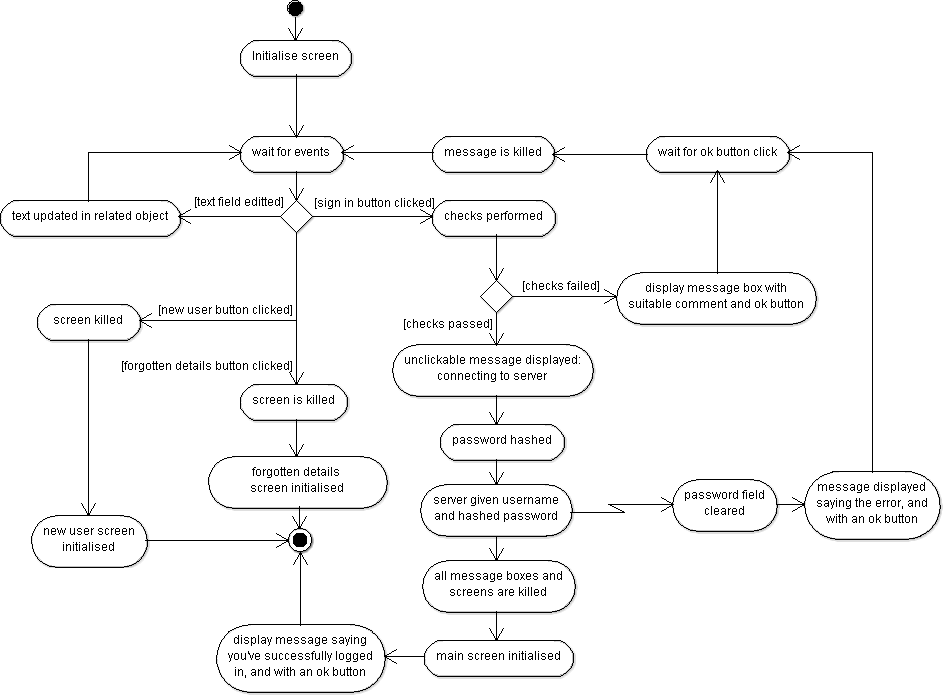
\includegraphics[width=\textwidth]{images/activity/main-login}
\end{figure}

When a user first starts the app they will be taken to the main login screen. Figure x shows what can happen from this screen. Firstly the screen is initialised and graphics, buttons and text fields are put in the grid that makes up the view. After this the app will wait for events from the user, these include typing into the text fields and clicking buttons. If text is typed it is saved in the relevant text field and if the new user button or forgotten details button are clicked then the main login screen is killed and the relevant screen is initialised. However if the sign in button is clicked, the following processes are a bit more complex. Firstly the text fields are checked and if they are null a message is displayed. This message box will have an OK button that once clicked will kill the message box and the app will wait for more events. If the text fields aren't empty then the password is hashed and the hash and username is given to the server. If there are any errors connecting to the server or creating the user session then a message box with be displayed with the error and an OK button. If not the user will be logged on and shown the main screen and a message box saying successfully logged on, with an OK button. This satisfies requirement 5.1.5 user authentication.

Similar processes will occur for creating a new account from the new user screen, except the checks performed include making sure text fields aren't null, the username and password are 5-16 characters long, the password and check password fields contain the same String as the email and confirm email fields, the password has a letter and digit and the email is valid. In this case the server will be given the username and email as well as the hashed password and if there are no errors with the server the user will be shown the main login screen with a message telling them that an email has been sent to them to activate their new account. This satisfies requirement 5.1.1 account registration.

There are also few differences when a user has forgotten their password and has clicked the forgotten password button. The email address text field must be checked to see if a valid email has been entered. If the server request is successful then the user will be shown the main login screen with a message telling them that an email has been sent to them with a link to refresh their password. This satisfies requirement 5.1.8 password reset.

\begin{figure}[h!]
    \centering
    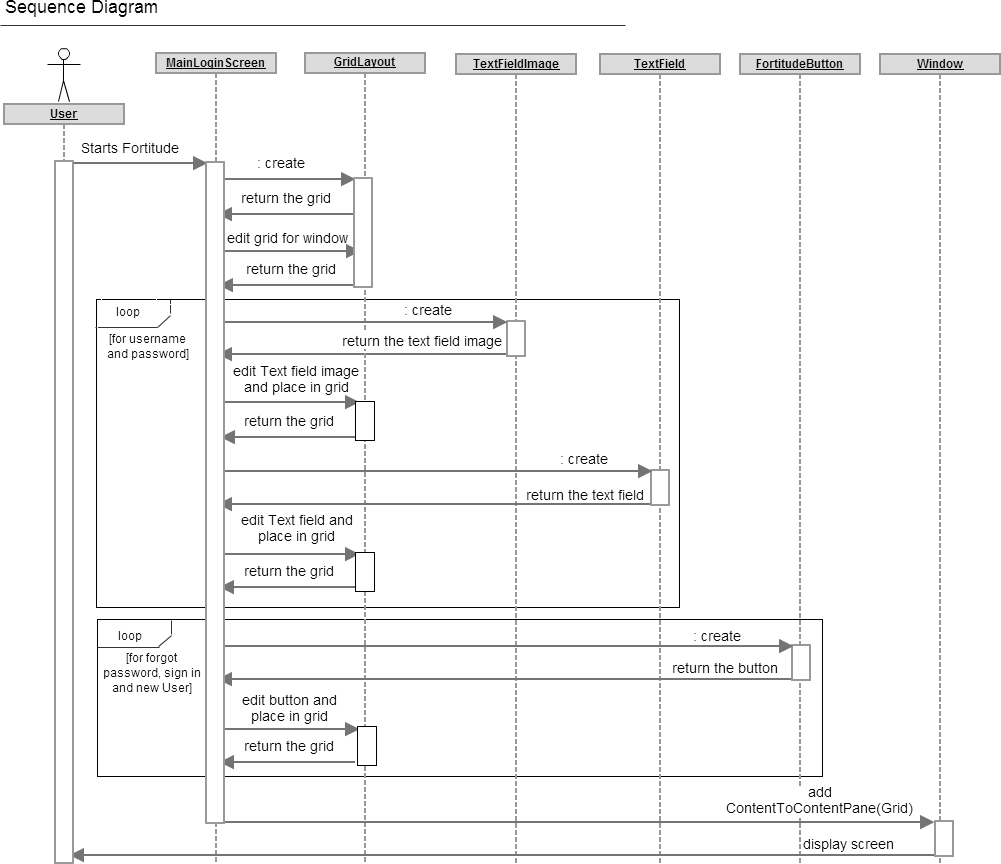
\includegraphics[width=\textwidth]{images/sequence/createMainLoginScreen}
\end{figure}

Figure x shows what happens in each of the classes when the main login screen is initialised. It is very similar for all screens. Once a new MainLoginScreen is created, the grid which everything sits on is initialised in the GridLayout class. The MainLoginScreen transforms the grid so it has enough squares and is the right size. Instances of TextFieldImage and TextField are initialised, edited and placed in the grid for username and password. Then the buttons for forgot password, sign in and new User are initialized in FortitudeButton, edited in the MainLoginScreen and placed in the grid. This grid is put in the window using a method in the Window class and this method displays the window to the user. When creating the grid and everything that goes in it the sizes are decided on the window size so nothing will be off the screen, satisfying requirement 5.3.8.

Figure x shows the sequence of events when the sign in button on the main login screen is pressed. Firstly the MainLoginScreen will call the method signIn(). It checks to see if the text fields aren't empty and displays a message box if they are. If not a message box saying connecting to server will appear which should satisfy requirement 5.3.9 as the rest may take a while to be performed but the user will see the message box nearly instantly. Next initialLogin() is called in the Login class which will hash the password and give the username and hashed password to ServerRequests. This will create an object of type RequestThread and call setURL() to give it a URL with all relevant information. This object connects to the server using the JSON parsing module and will analyse the response. JSON is used because it is very `light weight' to satisfy requirement 5.2.30. In the diagram I've just talked about a successful response. However if an error occurs the response will show this so ServerRequests can create a MessageBox with different text and not create a CurrentUser or display the main screen. But if the response is a success then these things will happen and a message with an OK button will be displayed that tells the user they've successfully logged on. This class diagram is very similar to other processes in the app as values are always checked in the current screen and the ServerRequests and RequestThread class as well as the JSON parsing module are used for most actions with a different method call in ServerRequests, therefore I will not include further class diagrams exactly how methods in ServerRequests work. Values are also checked by the server, however they are initially checked by the application as it will not take much processing time so the user will get a faster response if they've made a mistake.

\begin{landscape}
\begin{figure}
    \centering
    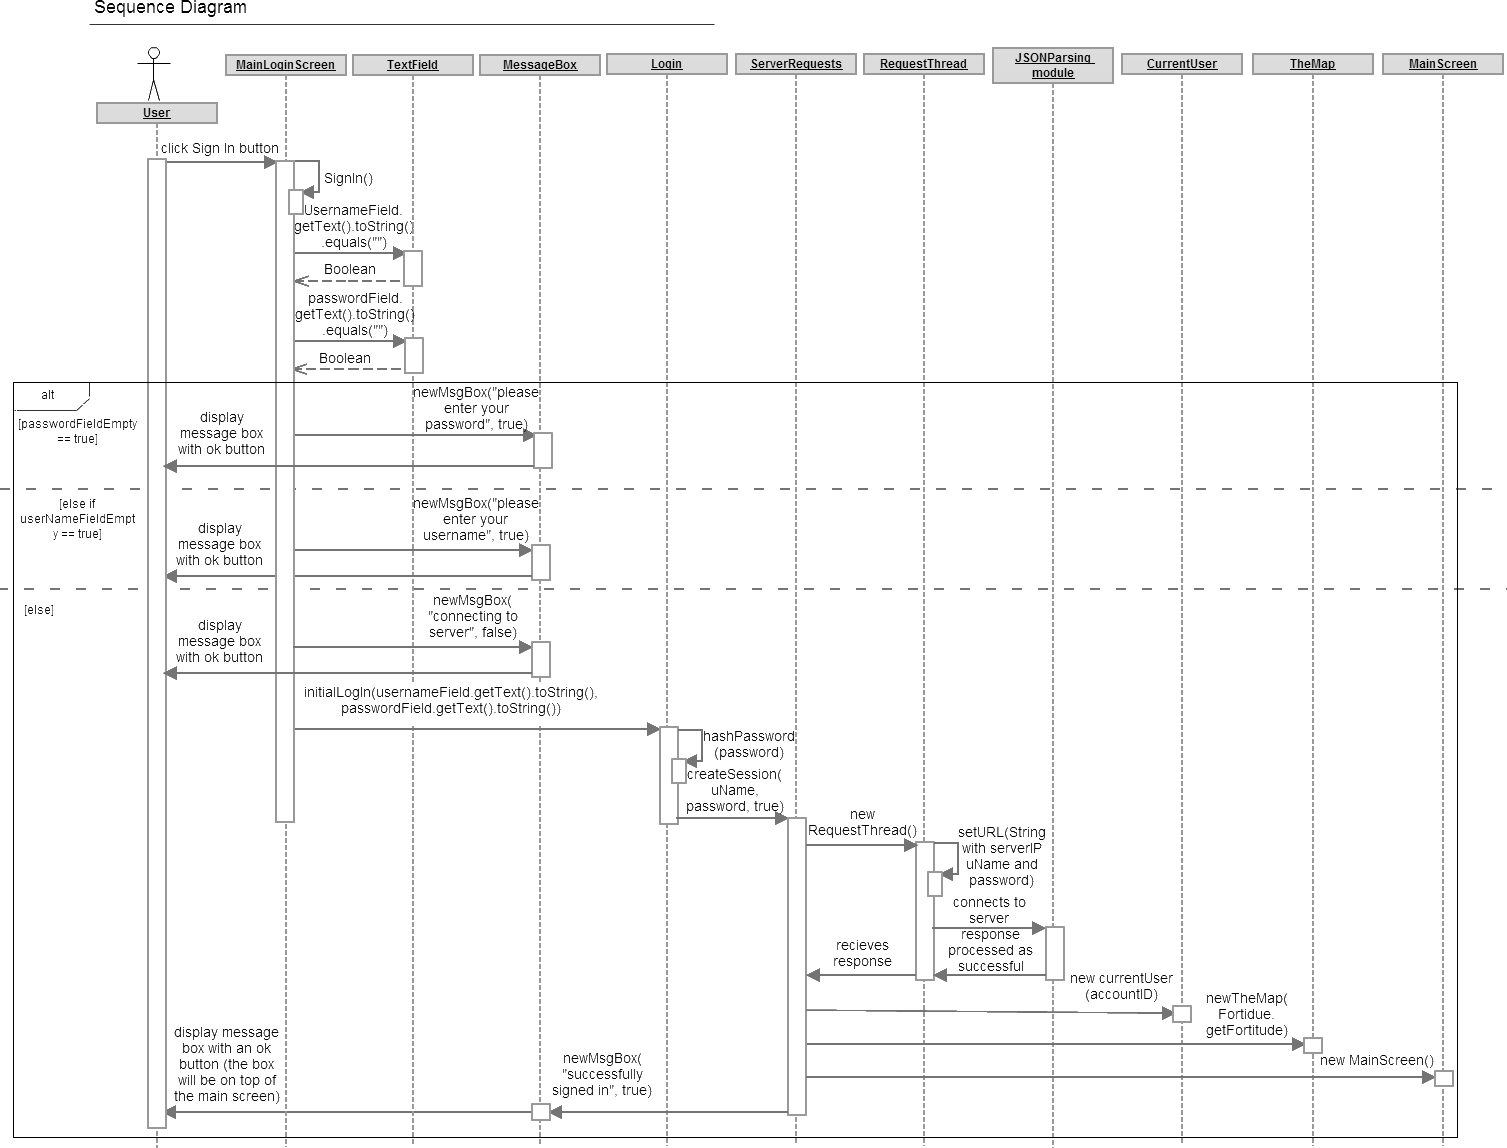
\includegraphics[height=\textwidth]{images/sequence/signInbutton}
\end{figure}
\end{landscape}

\begin{wrapfigure}{r}{0.6\textwidth}
    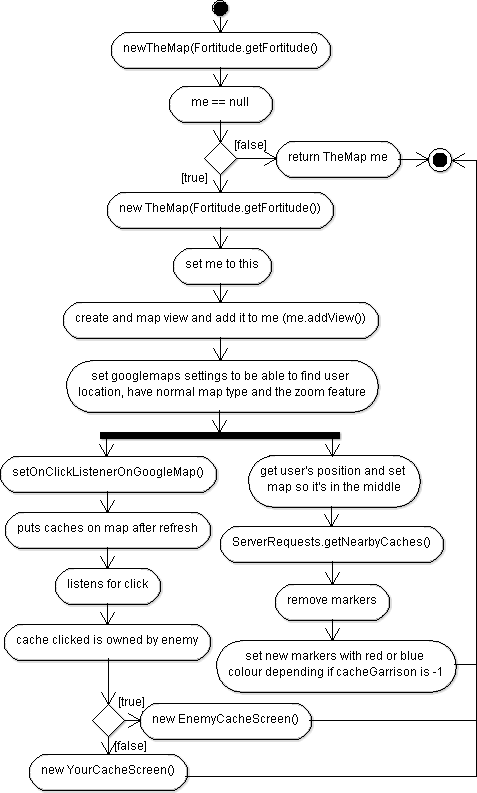
\includegraphics[width=0.6\textwidth]{images/activity/newMap}
\end{wrapfigure}

Before the main screen is shown the map must be created as it is viewed on the main screen. If it has already been created it is returned else a new map is created. When this happens a map view is created and added to the map and particular Google map settings are enabled, including zooming to satisfy requirement 5.3.3. Then threading is used to run two parallel processes, one gets the users position and set's the map to be showing this position, (satisfying requirement 5.3.1) get's nearby caches and set's them as markers on the map with different colours and types relating to owners and cache types, to satisfy requirement 5.2.26. This has a separate method so that caches can be loaded around the user's position when requested to satisfy requirement 5.3.2. When getting the nearby non-player caches, it will only put them on the map if the user hasn't attacked it for a certain amount of time, satisfying requirement 5.2.19. The other parallel process deals with user interactions, putting caches on the map after the user refreshes it and listens for when the user clicks a cache to bring up a new related screen.

If a user has logged on before they will be automatically signed into that account again as shown in figure x. After the MainLoginScreen has been initialised it will create an instance of FileSave and use it to get username and password hash in String form the byte form in files that the app stores. If the username and password aren't null or empty then the ServerRequests class can create a session for the user from them, and take the user to the main screen. However if the username and password are empty or null then nothing will happen and the user will not be told they are connecting to the server but shown the main login screen. When a user logs out through the AccountScreen, their username and password are put as the empty string using the createDialog() method in FileSave.

If a user's account is not already activated then the bottom bar in the main screen will not have the normal buttons but instead have a button to take the user to the ActivateUserScreen. From this screen the user can click a button to resend the activation email which uses resendActivationEmail() in ServerRequests with the email of the account. This satisfies requirement 5.1.4.

\begin{wrapfigure}{l}{0.7\textwidth}
    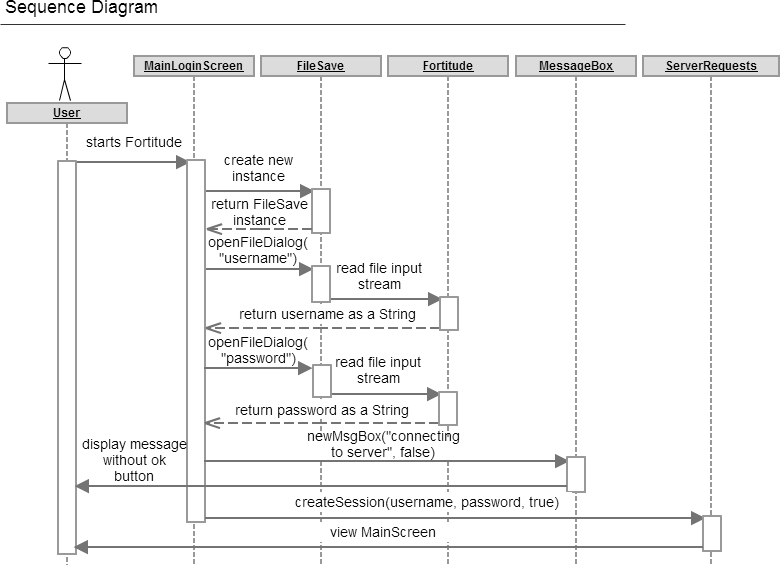
\includegraphics[width=0.7\textwidth]{images/sequence/autosave}
\end{wrapfigure}

\noindent
The sequence diagram for clicking the castle button is more complicated than for clicking other buttons so is shown in figure x. For these events to occur the castle button must be clickable. If the castle is clickable a message is shown telling the user they're being connected to the server. Then refreshData() is called in the ServerRequests class to make sure all information including cache positions and user data is up to date. refreshData() can update a route to a cache too if there is one. If this request isn't successful then a message with an OK button is displayed to the user that says loading caches failed. If the request is successful then the latitudes and longitudes are found out for the user's current position and caches on the map and nearest cache and distance to it is calculated. If the closest cache isn't close enough then user is shown a message box with an OK button that tells them to get closer to the cache. Otherwise if the cache is owned by them they go to the visit your cache screen, which will show the cache balance satisfying requirement 5.2.4. However, if the cache isn't owned by them they go to the visit enemy cache screen which will say the owner of the cache. If it's a non-player cache the visit enemy cache screen is still used, however it will not have the owner of the cache on. This will satisfy requirement 5.2.3, cache ownership.

\newpage
\begin{figure}
    \centering
    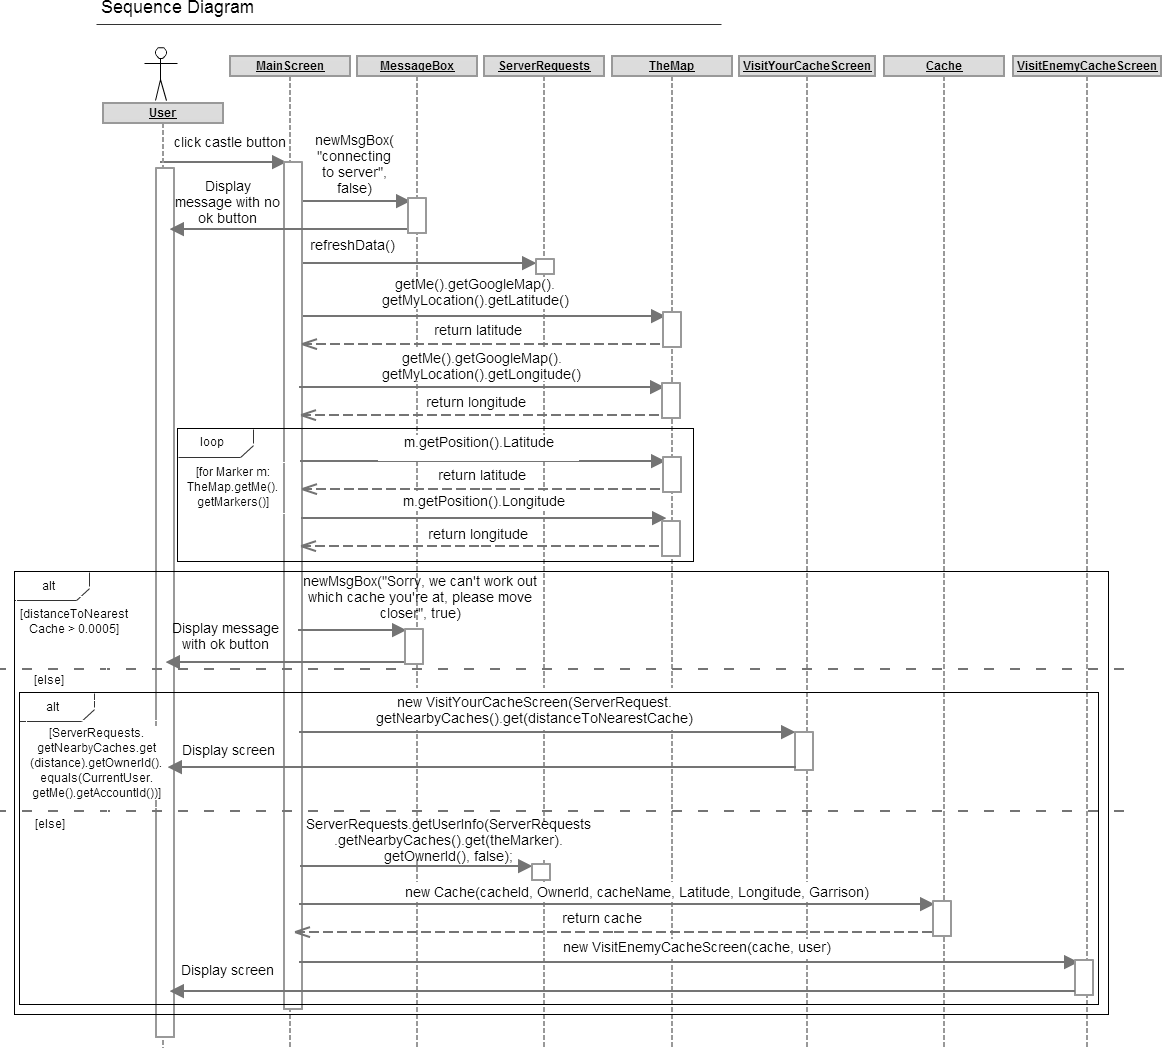
\includegraphics[width=\textwidth]{images/sequence/castleButton}
\end{figure}

As previously said the IconUpdater class decides whether the castle button is clickable and also what image is displayed for it. Once created, it runs in the background of the app unless it's told not to. While it hasn't been told to stop running it tries to get the position of the user and the positions of caches. If any cache is close enough then if the main screen is displayed the castle icon is viewed as not greyed out and made clickable. Else if no cache is close enough and the main screen is displayed the icon is viewed as greyed out and changed so when clicked nothing happens. If IconUpdater gets an error doing any of this more than 10 times the user is told that the IconUpdater has crashed through a message box.

\newpage
\begin{figure}
    \centering
    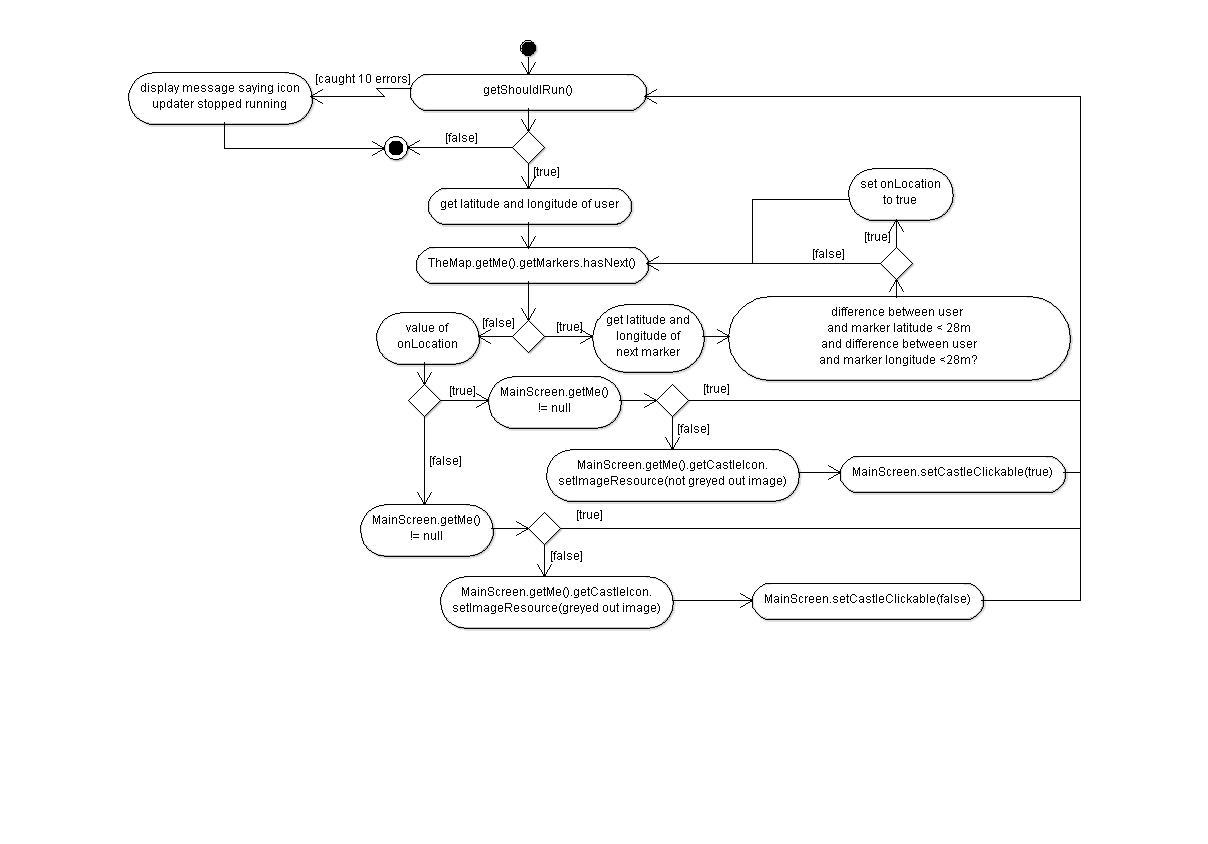
\includegraphics[width=\textwidth]{images/activity/iconUpdator}
\end{figure}

The castle button is used to attack and scout caches. When the scout cache button is clicked the app checks it can access the phone's location and Google maps. If it can't it will tell the user the problem else the user is told they are being connected to the server. The user sends a request to the server to scout a cache using the phone's location, the users chosen number of scouts to send and the cache ID. If there is a problem then it is explained to the user. The server is then asked to refresh the data so any scouts that are lost are updated on the app. Again the user is told any problems. When the first request was sent a response was made and the app analyses this to find out which screen to display next. If all the scouts sent were lost the scout failure screen is displayed else the scout success screen is displayed. This satisfies requirement 5.2.9 cache scouting.

\newpage
\begin{figure}
    \centering
    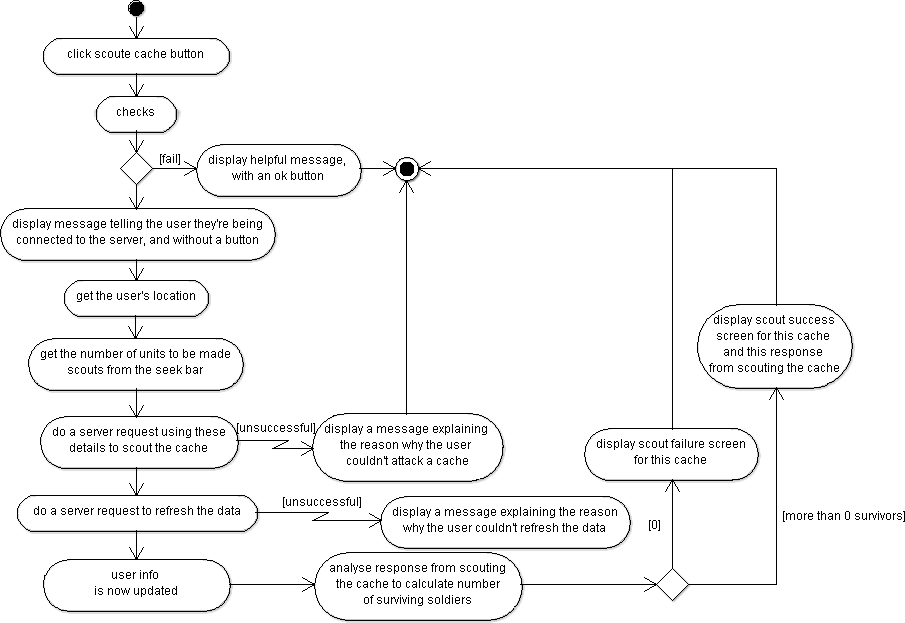
\includegraphics[width=\textwidth]{images/activity/scout-cache}
\end{figure}

A user can attack caches by clicking on an attack cache button. The app checks the location can be found and tells the user if their location can't be found. If it can be found the user is told they're being connected to the server. The user's location, number of units they wish to fight with and the ID of the cache are used to make a server request to attack a cache. The server is then requested to be refreshed so all the data can be changed based on the outcome of the attack such as the new cache balance from the remaining defenders or attackers and the owner of the cache. This satisfies requirements 5.2.11 successful attack and 5.2.12 successful defence. If there are any problems with these requests the user is told. If not the user is displayed the post battle screen which processes and displays the response from the first server request, which will satisfy requirement 5.2.13 battle breakdown. This satisfies 5.2.10 cache attacking. Attacking non-player caches is very similar, however the refreshing data might change whether or not the cache is viewed on the map if the user wins the battle, also the owner and cache balance will never change. This satisfies the requirements 5.2.17, 5.2.18, and 5.2.19.

\newpage
\begin{figure}
    \centering
    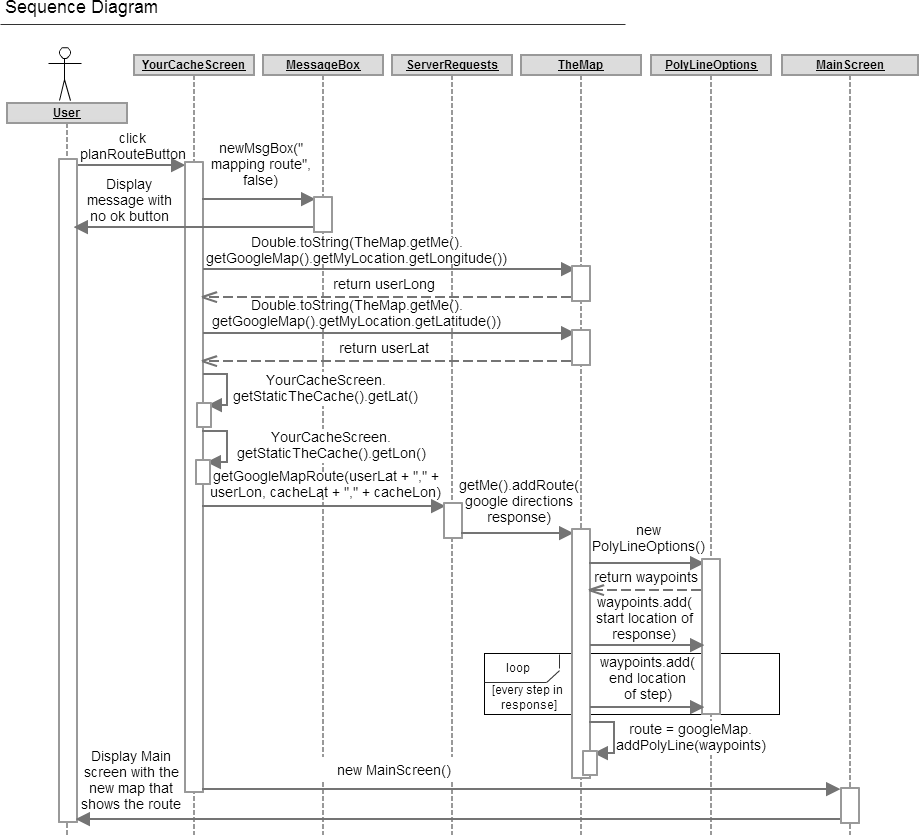
\includegraphics[width=\textwidth]{images/sequence/getRoute}
\end{figure}

A user can get to caches using a plan route button. In figure x I've used the one on YourCacheScreen as an example but you can similarly plan routes to enemy caches. Firstly when the user clicks the button their location is checked and if it can't be found they are told. If not they are told the route is being mapped. TheMap class is used to find the users location and the class of the screen they're on is used to find the caches location. The locations are used as Strings for the getGoogleMapRoute() method in the ServerRequests class. This calls the addRoute() method in TheMap class with the response received. This method uses a predefined class to create waypoints out of the response and join them up on the map to make a route. Lastly the user is taken to the MainScreen with the route on the map. This satisfies requirement 5.3.4 path finding.

\newpage
\begin{figure}
    \centering
    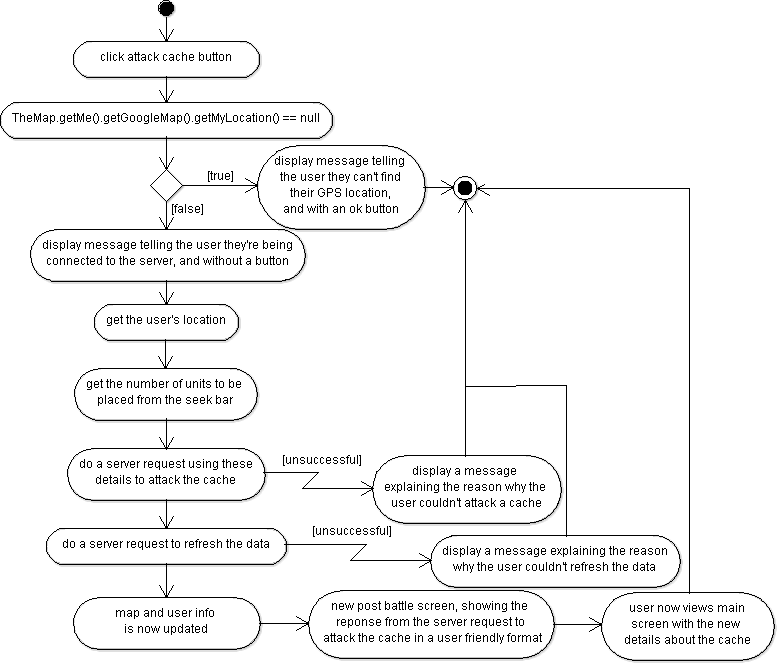
\includegraphics[width=\textwidth]{images/activity/attackCache}
\end{figure}

A user can place a cache by clicking the flag button. If their location can't be found they are told else they are told they're being connected to the server. A server request is made using the user's location and number of defenders they wish to make defenders for the cache to be placed. If this is unsuccessful e.g. due to an error or being too close to another cache then the user is told else the server is requested to refresh the data for the new cache to be added. Again if this is unsuccessful the user is notified why, else the user goes to a new main screen with the map now showing the cache. This satisfies requirement 5.3.5 cache placement. Note: when a cache is placed there must be at least 5 units in the seek bar, 4 of which will be lost. This satisfies requirement 5.2.8 cache placement cost.

\newpage
\begin{figure}
    \centering
    \includegraphics[width=\textwidth]{images/activity/placeCache}
\end{figure}

On the cache transactions screen the user can withdraw and deposit soldiers from the cache. When the submit button is pressed the users location will be found and if it's null then the user will be displayed an error message, if not they will be told they're being connected to the server. The number of units to be withdrawn or deposited will be found from the seek bar, ServerRequest.cacheTransactions() will be called then ServerRequests.refreshData(), to be able to view the changed balances. If any errors occur in the ServerRequest methods then the user will be explained the error in a message, else they'll be taken back to the main screen. This will satisfy requirement 5.2.5, and 5.2.7. If the user withdraws all the troops then the cache will become unowned satisfying requirement 5.2.6. Unowned caches will have a separate screen from which users can place soldiers in to own that cache, further satisfying requirement 5.2.7.

There is a messaging feature in the app, which can be navigated around from the inbox screen. This screen will be made like most other screens except for the buttons to particular messages, where a few more classes need to be involved before adding these to the grid. Firstly the information about the 7 viewable messages are set using ServerRequests.setMessages(username, when). The when variable is used to tell which 7 messages are used, for example if the user clicks next twice then the 3rd set of 7 messages will be used, then if the user clicks previous the 2nd set of 7 messages will be used. There will be checks in place to stop `when' being invalid for example negative or so large there are no messages in the set. The message information is used to decide what the icons look like and the text displayed. This satisfies requirement 5.4.1 user communication.

\begin{figure}
    \centering
    \includegraphics[width=\textwidth]{images/sequence/inbox}
\end{figure}

When a user clicks an icon to go to a message the variables related to currentMessage are set to those from the corresponding message in the array in the Messages class and if currentMessage.getRead() is false then ServerRequest.setRead(currentMessageID) is called and currentMessage.setRead(true). The values in currentMessage are then used to view the message screen, to automatically put the correct user in the `send to' box when replying and to feed into the server request reportMessage if a user wishes to report the message. This satisfies requirement 5.4.2 communication reporting.

Cache reporting works much like message reporting and is done through the same screen. When reporting a cache, the screen will have a subject and description relating to caches rather than messages, and when submit is pressed reportCache() in ServerRequests will be called with the cache, the user and the text that was entered as parameters. This satisfies requirement 5.2.22 cache reporting.

Users can block other users through the settings menu in messages and through the EnemyProfileScreen account screen. When a user is blocked, User.getBlockedUsers() is called to check if the user is already blocked and if not User.addBlockedUser(String username) is called then the method blockUser(String userBlocker, String userBlocked) is called in ServerRequests. The information is stored in the app and server as it will speed up loading screens to have it in the app while it has to be in the server so when other users messages aren't sent they can be notified. When a user is unblocked, the User class checks they are blocked are removes them from the list of blocked users using User.removeBlockedUser(String username), then the method unBlockUser(String userBlocker, String userBlocked) is called in ServerRequests. A user is blocked and unblocked using the same button in the EnemyProfileScreen so when this screen is made and the button is pressed User.getBlockedUsers().contains(String username) must be called to decide which button is displayed and what action is taken. In the settings menu of messages a list of blocked users are displayed so whenever this screen is initialised the User class is used to find the names and whenever a user is blocked or unblocked the screen must be reloaded. When a user sends a message to a blocked user, the message will still be sent to and stored in the server however the user will be shown a message box saying the message was unable to send.

There is a recent news screen which works much like the inbox screen. When it is initialised setActivity(String username, int when) from the serverRequests class is called to add the information needed from the server. It creates button rows that have different text and icons using this information. It also stores the JSON responses on the app so that when a row is clicked the user can go to the right screen. If the boolean corresponding to the row clicked in isMessage is false then the cache is extracted from the corresponding response using get(``cache'') and this and the response is used to display the post battle screen. If the corresponding value in the isMessage array is true then values for sender, subject and body are extracted and stored as the corresponding current message variables in the Messages class and used to view the message screen. This satisfies requirement 5.3.6 activity recording.

\begin{figure}
    \centering
    \includegraphics[width=\textwidth]{images/activity/recentActivity}
\end{figure}

Special caches will involve the SpecialCacheUpdate class that works much like the IconUpdator class. It is constantly running in the background, getting user's WiFi networks and checking if any have a MAC address of a special cache. If the user can connect to a particular MAC address, then if they are currently on the main screen, the screen will be killed, and the user will be shown the SpecialCacheFoundScreen. From here they can click to claim their prize and if they can still connect to the network with the right MAC address and the reward is still available, they will be displayed a message telling them they were successful, their account will be refreshed so the server knows not to use this special cache in the SpecialCacheUpdate again and the users balance will be updated, which will satisfy requirement 5.2.2 and 5.2.21. If they can no longer connect to the correct network they will be displayed a message saying they were unsuccessful. Either way they will then be taken back to the main screen. This will satisfy requirement 5.2.20, special event placement.

As you can see after user actions that could change data, the data is refreshed which means it will be accurate so a user can see their account balance accurately at any time satisfying requirement 5.2.1 and points can be added or removed from an account balance by other components of the system satisfying requirement 5.2.2. As all user actions involve displaying a message box requirement 5.2.14 cache operation chronology will be satisfied because a message box disables the screen underneath, so the user can't do anything else until the server has finished processing the action.

This section will now take a look at the design of the server. When a request is made in general, the processes in figure x will occur. The APIManager class will receive a URL from an external source in a form such as /api/scout?uname=Metapyziks\&session=0123456789abcdef. It will use the Request class to find the specific request class needed so in this case it would be the ScoutCacheRequest class. It will then use the method Respond in the specific request class to get a response that is changed into JSON form and sent back to the external source. However if a specific request class can't be found then the ErrorResponse class is used. The server is not going to involve threading so each task will be carried out one at a time to satisfy requirement 5.2.14.

\begin{wrapfigure}{l}{0.65\textwidth}
    \includegraphics[width=0.65\textwidth]{images/sequence/Servergeneral}
\end{wrapfigure}

The following sequence diagram shows how the specific request class RegisterRequests is used to get a response. Firstly the method attemptRegister() is called in the account class. This method will perform the checks needed to satisfy requirement 5.1.1. If any of these checks are failed then a related instance of ErrorResponse will be returned. If the checks are passed then a new account will be made with the username, email and password hash supplied, the rank as unverified, the registration date set to the current time, the activities list set to a new list of Response, the blocked list as a new list of String and the dictionary of non-player caches found created. (The rank can be changed to Administrator which satisfies requirement 5.1.3) This account is placed in the database and used as a parameter in EmailValidationCode.create() along with the Enum EmailValidationType set to Activate. The code created is used to send an email to the user to activate their account, which will satisfy requirement 5.1.2. If it has got to this point in the method then null is returned so the Response is made using the Response method which gives a successful response rather than an error.

\begin{figure}
    \centering
    \includegraphics[width=\textwidth]{images/sequence/registerUser}
\end{figure}

\begin{wrapfigure}{r}{0.5\textwidth}
    \includegraphics[width=0.5\textwidth]{images/sequence/userinfo}
\end{wrapfigure}

When resending an activation email it is the SendActivationRequest class that performs checks to satisfy requirement 5.4.1. The account with the email address provided is selected from the database and used to resend an activation email in the same way as account registration. If an ErrorResponse hasn't already been returned then a Response will be like with account registration.

When sending a password reset email, PasswordResetRequest let's EmailValidationCode perform the checks to satisfy requirement 5.1.8 in the method AttemptCreate(). If it passes these checks an EmailValidationCode will be created and used to send an email to the user and a Response will be returned, else if the checks aren't passed an ErrorResponse will be returned.

Figure x shows how UserInfoRequest works, as you can see the checks are performed in the specific request class. If passed then the accounts and caches of the users wanted are found. The response is found using this list of Account and a list of Int corresponding to the number of caches the user has. UserInfoResponse uses these parameters to make a response in the form:

\begin{verbatim}
{"users":[{"accounted":0,"uname":"metapyziks","regdate":1347374370,
"rank":Unverified,"caches":0},{"accounted":1,"uname":"TestName",
"regdate":1347381045,"rank":Verified,"caches":23}],"success":true}
\end{verbatim}

\begin{wrapfigure}{l}{0.6\textwidth}
    \includegraphics[width=0.6\textwidth]{images/sequence/createSession}
\end{wrapfigure}

The server creates a new session using StartSessionRequest. This performs all the necessary checks on the username, email, password hash supplied with the Request class, which will also get the account corresponding to the user supplied and check the account along with the SessionInfoResponse corresponding to the account. It checks expiration using the method IsExpired() in AuthSession. If any of the checks are failed a related ErrorResponse is initiated and fail is returned to StartSessionRequest which will not go on to do AuthSession.Create(account). If the checks are passed the instance of AuthSession is refreshed which will set the refresh time to the current time so it can be used in the IsExpired() method. True is returned to StartSessionRequest, a new instance of AuthSession is made with an AccountID, SessionCode, LastRefresh set to now and a Rank set to the rank of the account. The AuthSession is added to a dictionary of AuthSession as an update or new entry with a new AccountID. The AuthSession is returned to StartSessionRequest which is used to create a new SessionInfoResponse with a code and success value. This satisfies requirement 5.1.5 user authentication.

The UserStatsRequest class works by checking in the same way as StartSessionRequest using CheckAuth(). If the checks are passed an instance of Player is created using Player.GetPlayer(account), which selects the player in the database with the correct AccountID using Select() in DatabaseManager. If this player doesn't exist yet then a new Player is created with a balance of 0 and AccountID then inserted into the database using Insert() in DatabaseManager (see scouting figure). The caches the user owns are found using Select() with the caches AccountID as the as the account's AccountID. caches.Sum() is used to find the number of points stored in all the caches owned by the account holder and this along with the player Balance and cache Count is used to create a new UserStatsResponse. This satisfies requirement 5.2.1, account balance.

To list a users' caches, UserCachesRequest is used, which uses CheckAuth() to find errors. If there aren't any errors then a list of Cache is found with the same AccountID as the Account of the specified user using DatabaseManager. The response including the caches' cacheid, ownerid, name, latitude, longitude and garrison is found by new CacheInfoResponse(caches).

To find a list of nearby caches, NearbyCachesRequest is used. This firstly find errors with CheckAuth() then if none are found it will check the latitude, longitude and radius can be parsed as a double and if not make a new related ErrorResponse. Else that latitude, longitude and radius are used for Cache.FindNearby() which uses DatabaseManager.Select() to find a list of Cache in the radius. The balance of the caches not owned by the user are set to -1 so the user can't know about enemy garrisons, satisfying requirement 5.2.4 cache balance. The balance of non-player caches is set to -2 to make them distinct from other caches, and they will only be put in the response if the user hasn't defeated the cache in a certain amount of time, satisfying requirement 5.2.19. Again CacheInfoResponse is used if there wasn't an ErrorResponse needed. This satisfies requirement 5.3.2 nearby caches.

When a cache is scouted, the ScoutCacheRequest class is used. Checks's are made using checkAuth(), by trying to parse the Strings representing numbers (e.g. units and latitude) into Doubles, and by seeing if the numbers are in the right bounds e.g. positive or smaller than the user's balance. Tools.getDistance() uses trigonometry to find the distance between the user and closest cache. Tools.CoinToss used to calculate the survivors, it creates a random number and if this number is less than 0.8, true is outputted. This is done for every soldier in the scouting army and the number of trues outputted equals the number of survivors. The players balance is set to balance – units + survivors and this is updated in the database. A new ScoutCacheResponse is made with the CacheID, Scouts set to units, Survivors and Garrison set to cache.Balance. The response will include cacheid, ownerid, cache name, latitude, longitude, garrison and success. The response will be put in Activity, the list of responses in the corresponding Account class and updated in the database. This satisfies requirement 5.2.9 cache scouting.

\begin{figure}
    \centering
    \includegraphics[width=\textwidth]{images/sequence/scoutCache}
\end{figure}

The PlaceCacheRequest class performs checks much like the ScoutRequest class, it does CheckAuth(), CheckLocation(), checks units are a Double, larger than the CachePlacementCost and smaller than the player's balance. CheckLocation() see's if the location hash supplied is the same as the location given which will satisfy requirement 5.2.24 anti-cheating measures. It also uses Cache.FindNearby() which uses as supplied minimum distance, latitude and longitude to find the caches within that distance, and PlaceCacheRequest uses this information to see if the user is far enough away from other cache to place a cache. If all of the checks are passed then a new Cache is made with an AccountID, Balance which is 4 less than units, Latitude, Longitude, Name which is randomly selected, CacheID which isn't supplied by PlaceCacheRequest and Nonplayer set to false. The Cache has an associated AccountID to satisfy requirement 5.2.3, cache ownership, and a Balance to satisfy requirement 5.2.4 cache balance, which is less than units to satisfy requirement 5.2.8 cache placement cost. The players balance is updated and saved in the database, and the cache and activity is inserted into the database. A new CacheInfoResponse is made which includes cacheid, ownerid, name, latitude, longitude, garrison and success. This satisfies requirement 5.3.5 cache placement.

\begin{figure}
    \centering
    \includegraphics[width=0.7\textwidth]{images/activity/server_attackCache}
\end{figure}

As you can see the checks for attacking caches are done in the AttackCacheRequest class, and the response is created in the Cache class. The sum used for weight is based off research (ASK EMMA FIGURES). The BattleReportResponse is initially set with the cache, AttackerID, DefenderID, Attackers made from a new BattleReportResponse.UnitReport with Initial and Survivors set to units, and Defenders made from a new BattleReportResponse.UnitReport with Initial and Survivors set to cache Balance. The fatalaties are put in the report with report.Attackers.Fatalities = report.Attackers.Initial – report.Attackers.Survivors and a similar method for Defenders. Report.IsVictory is true if there are attacking survivors, in this case report.Attackers.Deserters = 0 while the defending deserters are a small random proportion of the defending fatalities, the cache Balance becomes the surviving attackers plus the defending deserters and the caches AccountID becomes the attackers AccountID. However if IsVictory is false, there are 0 defending deserters, a small proportion of the attacking fatalities are deserters, the cache balance is the surviving defenders and the attacking deserters are added to the defenders balance. The response is added to Activity in the affected instances of Account and updated in the database. This satisfies requirement 5.2.10 cache attacking, 5.2.11 successful attack, 5.2.12 successful defence and 5.2.13 battle breakdown. Attacking non-player caches is very similar, the same request is used, the only difference is that the user's Account NonPlayerDictionary will be updated with the cacheID and time, the `point reward' will be shown as the deserters, which there will be more of to make up for not getting the cache, and the cache balance won't change in the database. This satisfies requirement 5.2.18.

When a message is sent the MessageRequest class is used, it checks the message body and subject aren't empty. It will create a MessageResponse and put it in Activity of the sender's and receiver's Account and updated on the database. It will check the receiver's Account to see if the sender is blocked and return an ErrorResponse if the sender is blocked else a Response is returned. This satisfies requirement 5.4.1.The receiver will always get the message as it is when the activities are requested that the server will make sure that messages aren't received from blocked users. This is so that when a user is unblocked the messages will be received and in the correct order in relation to other activities. There will obviously be a request to block users too which will check the username or id supplied has an associated account that isn't the account of the user before adding the id to the Block list in the user's account. The possible responses are the ErrorResponse or Response. The request to unblock a user is the oppositeto blocking users.

Messages and caches will be able to be reported through the MessageReportRequest and CacheReportRequest classes. They will use the reporterid or username, message or cache id, and a description. They will check the cache or message hasn't previously been reported, and if it's a CacheReportRequest then that it's not the reporter's cache and it's not a non-player cache. The message id is searched for in the reporter's activity to find the message details, or the cache details are found using the cacheid. This information is put into a related Response and added as an AdminResponse in the database so administrators can see it on the website. The cache or message will be marked as reported and saved in the database and a Response will be returned. This satisfies requirement 5.2.22 and 5.4.2.

In many requests the DatabaseManager and Account classes are used in conjunction with the specific request class, with this requirement 5.2.2. Account Transactions and 5.3.6 Activity Recording can be fulfilled. There will also be a Request class for getting activities that uses the users Account ID or username, how many activities they wish to see, which set of they want, and what type. It performs checks (including removing messages from blocked user's from the response) and uses modular arithmetic to select the correct set of activities of the right type and return them in ActivityResponse. Requirement 5.2.5 cache transactions is fulfilled in the same way as 5.2.2 but with Cache class, the request used to withdraw and deposit soldiers will also set the cache owner to null and update it in the database if all the soldiers are withdrawn. This will satisfy requirement 5.2.6.

\begin{wrapfigure}{r}{0.58\textwidth}
    \includegraphics[width=0.58\textwidth]{images/activity/IndexHTML}
\end{wrapfigure}

The design of the website will now be discussed. Although not all pages are mentioned, the pages not mentioned will feature forms, checks and updates much like the pages which are examined in detail. This will satisfy requirement 5.4.3.

The index page is made as followed, firstly the header is used to find information needed. It includes function.html which provides a list of methods used for checking such as isAdmin() and pluralify(). If the Account of the user is verified then the Player and Cache classes are used to find the player and their caches. If the account has the rank admin or higher the admin panel is displayed along with the header everyone can see. If the session isn't null (ie isSignedIn()) then the side bar is personalized, and if the player and caches aren't null it is personalized further with the number of caches and the players balance. If the account is verified and there is a session then caches and news plus links to further information, caches and news are displayed in the sidebar. This sidebar will satisfy requirement 5.4.5 and 5.3.6. The links to caches will display pages that satisfy requirement 5.4.6.

\begin{landscape}
\begin{figure}
    \centering
    \includegraphics[width=1.2\textheight]{images/activity/loginWeb2}
\end{figure}
\end{landscape}

When a user logins in with the website login.html is used. It's head uses the username and password in the form to attempt to login, which will output a session. If the session outputted by Account is null a new session is made using cookies. The title is set and if necessary JavaScript is loaded for hashing passwords. The top bar is added, the subtitle set to Login. If there's an error then it is explained and a link is displayed to try again. If the session is null a form is produced for the user to enter their username and password, which will be hashed. A link is also provided in the case that the user forgets their password. If the session is not null then text will be displaying saying successfully logged in. This will satisfy requirement 5.4.4.

When a user clicks a link in an email to activate their account activate.html is used. In the head, there will be AttemptActivate(get["email"], get["code"] ) and the title will be set to Fortitude Server – Account Activation. In the body, a sub-title will be set as Account Activation. If AttemptActivate outputted an error that wasn't null then the user is explained the error, if not the user is told their account has been activated and they can now log on. A link will be provided to the Home page at the bottom of the body. This will satisfy requirement 5.1.2, account activation.

Admins can place a cache with placecache.html. In the head this checks whether this session is null and the rank of the session. If the session is null or the rank less than administrator the user is redirected to the error page. Else the account corresponding the username submitted is found and checked, if anything fails an error message is set. Else a new Cache is created and updated in the database. The title is set to Place Cache and a form is created to input username, latitude, longitude and units. If success is true then text is displayed saying where the cache was placed else if there was an error, the message is displayed. This satisfies requirement 5.2.16. placenon-playercache.html is very similar except the form will only include inputs for position and units. The cache created and added to the Server will have the AccountID as the administrator's AccountID. placespecialEvent.html is also similar, in the head it will be checked if the supplied MAC-address is valid and the number of user claiming the reward and the reward is greater than 0.

These will be in the form in the body. Then the special event cache will be placed in the database. This satisfies requirement 5.2.20.

Administrators can delete caches using deletecache.html, this will redirect the user to the error page if their session is null or rank not high enough. It will use the cacheid in the form to get the cache from the database, which will be checked to exist then removed from the database. If it doesn't exist then the error String will reflect this. Text is set to Delete Cache and a form is created for the user to submit Cache ID. If success is true the user is told which cache was successfully removed by name and cacheid. However if there was an error text is set to this error. This satisfies requirement 5.2.23. deleteAccount.html works in a very similar way, it is an admin only page and when the account is removed from the database, all the caches with the accountID are found and removed from the database too. This satisfies requirement 5.1.7. Users can also delete accounts through the website then the email they will receive from an administrator. Once the link in the email is clicked on the users' caches as well as account will be removed from the database.

\begin{figure}
    \centering
    \includegraphics[width=\textwidth]{images/activity/admin-placecache}
\end{figure}

\end{document}
